%% LyX 2.3.4.2 created this file.  For more info, see http://www.lyx.org/.
%% Do not edit unless you really know what you are doing.
\documentclass[english,dvipsnames,aspectratio=169,handout]{beamer}
\usepackage{mathptmx}
\usepackage{algorithm2e}
\usepackage{eulervm}
\usepackage[T1]{fontenc}
\usepackage[latin9]{inputenc}
\usepackage{babel}
\usepackage{amstext}
\usepackage{amssymb}
\usepackage{graphicx}
\usepackage{ifthen}
\usepackage{xcolor}
\usepackage{xspace}
\usepackage{tikz}
\usetikzlibrary{tikzmark}
\usetikzlibrary{calc}
\usepackage{pgfplots}
%\pgfplotsset{compat=1.17}
\usepackage{booktabs}
\usepackage{xpatch}
\usepackage{multirow}
\usepackage{colortbl}
\usepackage{pgfpages}
\usepackage{bbm}


\newcommand{\commenteq}[1]{{\color{brown}#1}}

\xpatchcmd{\itemize}
  {\def\makelabel}
  {\ifnum\@itemdepth=1\relax
     \setlength\itemsep{2ex}% separation for first level
   \else
     \ifnum\@itemdepth=2\relax
       \setlength\itemsep{1ex}% separation for second level
     \else
       \ifnum\@itemdepth=3\relax
         \setlength\itemsep{0.5ex}% separation for third level
   \fi\fi\fi\def\makelabel
  }
 {}
 {}

\ifx\hypersetup\undefined
  \AtBeginDocument{%
    \hypersetup{unicode=true,pdfusetitle,
 bookmarks=true,bookmarksnumbered=false,bookmarksopen=false,
 breaklinks=false,pdfborder={0 0 0},pdfborderstyle={},backref=false,colorlinks=true,
 allcolors=NYUPurple,urlcolor=LightPurple}
  }
\else
  \hypersetup{unicode=true,pdfusetitle,
 bookmarks=true,bookmarksnumbered=false,bookmarksopen=false,
 breaklinks=false,pdfborder={0 0 0},pdfborderstyle={},backref=false,colorlinks=true,
 allcolors=NYUPurple,urlcolor=LightPurple}
\fi

\makeatletter

%%%%%%%%%%%%%%%%%%%%%%%%%%%%%% LyX specific LaTeX commands.
%% Because html converters don't know tabularnewline
\providecommand{\tabularnewline}{\\}

%%%%%%%%%%%%%%%%%%%%%%%%%%%%%% Textclass specific LaTeX commands.
% this default might be overridden by plain title style
\newcommand\makebeamertitle{\frame{\maketitle}}%
% (ERT) argument for the TOC
\AtBeginDocument{%
  \let\origtableofcontents=\tableofcontents
  \def\tableofcontents{\@ifnextchar[{\origtableofcontents}{\gobbletableofcontents}}
  \def\gobbletableofcontents#1{\origtableofcontents}
}

%%%%%%%%%%%%%%%%%%%%%%%%%%%%%% User specified LaTeX commands.
\usetheme{CambridgeUS} 
\beamertemplatenavigationsymbolsempty


% Set Color ==============================
\definecolor{NYUPurple}{RGB}{87,6,140}
\definecolor{LightPurple}{RGB}{165,11,255}


\setbeamercolor{title}{fg=NYUPurple}
\setbeamercolor{frametitle}{fg=NYUPurple}

\setbeamercolor{background canvas}{fg=NYUPurple, bg=white}
\setbeamercolor{background}{fg=black, bg=NYUPurple}

\setbeamercolor{palette primary}{fg=black, bg=gray!30!white}
\setbeamercolor{palette secondary}{fg=black, bg=gray!20!white}
\setbeamercolor{palette tertiary}{fg=gray!20!white, bg=NYUPurple}

\setbeamertemplate{headline}{}
\setbeamerfont{itemize/enumerate body}{}
\setbeamerfont{itemize/enumerate subbody}{size=\normalsize}

\setbeamercolor{parttitle}{fg=NYUPurple}
\setbeamercolor{sectiontitle}{fg=NYUPurple}
\setbeamercolor{sectionname}{fg=NYUPurple}
\setbeamercolor{section page}{fg=NYUPurple}
%\setbeamercolor{description item}{fg=NYUPurple}
%\setbeamercolor{block title}{fg=NYUPurple}

\setbeamertemplate{blocks}[rounded][shadow=false]
\setbeamercolor{block body}{bg=normal text.bg!90!NYUPurple}
\setbeamercolor{block title}{bg=NYUPurple!30, fg=NYUPurple}



\AtBeginSection[]{
  \begin{frame}
  \vfill
  \centering
\setbeamercolor{section title}{fg=NYUPurple}
 \begin{beamercolorbox}[sep=8pt,center,shadow=true,rounded=true]{title}
    \usebeamerfont{title}\usebeamercolor[fg]{title}\insertsectionhead\par%
  \end{beamercolorbox}
  \vfill
  \end{frame}
}

\makeatother

\setlength{\parskip}{\medskipamount} 

\input ../macros

\begin{document}
\input ../rosenberg-macros

%\setbeameroption{show notes on second screen}

\title[CSCI-2565]{Decision Trees and Boosting}
% \author{Tal Linzen\\
% Slides based on Lecture
% \href{https://github.com/davidrosenberg/mlcourse/blob/gh-pages/Lectures/10.trees.pdf}{10} from David Rosenberg's course materials (\url{https://github.com/davidrosenberg/mlcourse})
% }
\author{Mengye Ren}
\date{Nov 14, 2023}
\institute{NYU}

\makebeamertitle
\mode<article>{Just in article version}

% \begin{frame}
% {Overview}
% \begin{itemize}
% \item Our first inherently non-linear classifier: decision trees.
% \item Ensemble methods: bagging and boosting.
% \end{itemize}
% \end{frame}

% \section{Decision Trees}

% \begin{frame}{Regression trees: Predicting basketball players' salaries}
%     \begin{minipage}{0.45\textwidth}
%         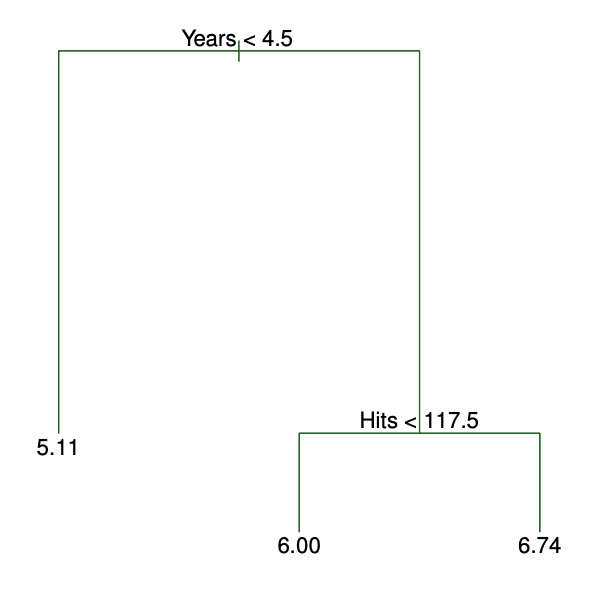
\includegraphics[width=\textwidth]{figures/basketball_decision_tree}
%     \end{minipage}%
%     \begin{minipage}{0.45\textwidth}
%         \pause
%         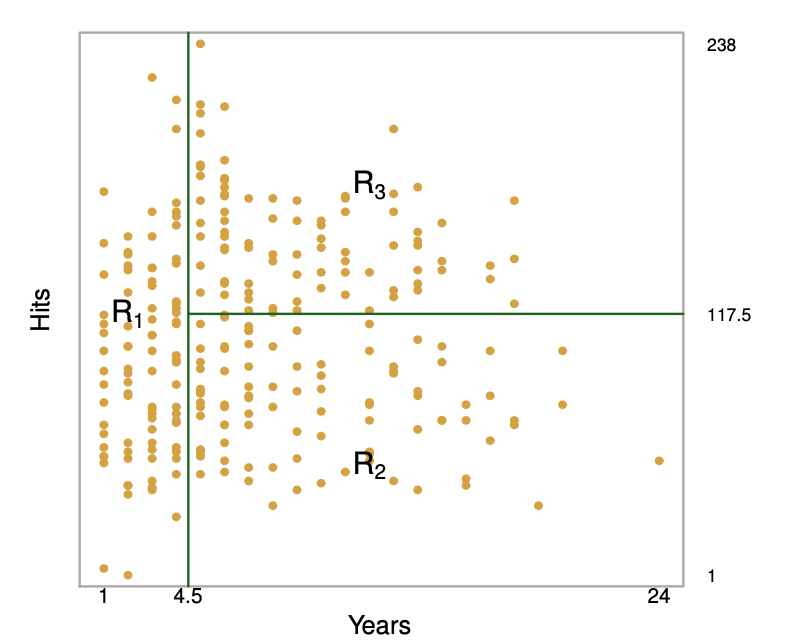
\includegraphics[height=\textwidth]{figures/basketball_regions}
%     \end{minipage}
% \end{frame}

% \begin{frame}{Classification trees}
% %\item Decision tree is a \textcolor{blue}{non-linear} classifier
% \begin{center}
% 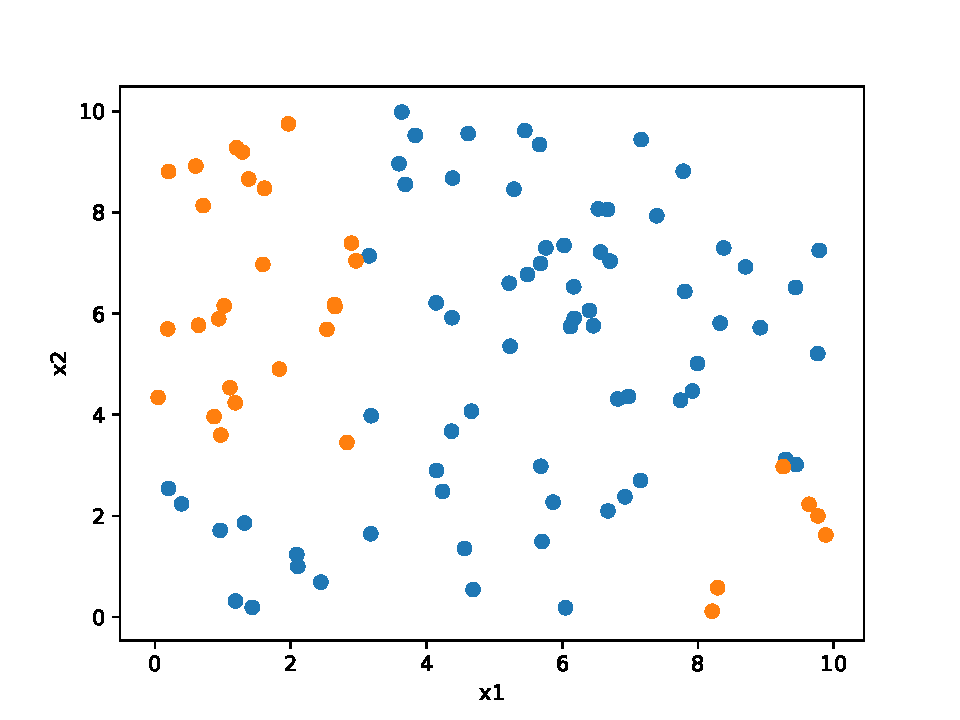
\includegraphics[height=0.6\textheight]{figures/dt-2d}
% \end{center}
% \begin{itemize}
% \item Can we classify these points using a linear classifier?
%     \pause
% \item Partition the data into axis-aligned regions \textcolor{blue}{recursively} (on the board)
% \end{itemize}
% \note[item]{Let's consider the dataset shown in the figure. How should we classify the orange and the blue points?}
% \note[item]{They are not linearly separable, but they belong to different regions. (draw regions)}
% \note[item]{Let's partition the space recursively.}
% \end{frame}

% \begin{frame}
% {Decision trees setup}
% \begin{columns}
% \begin{column}{0.5\textwidth}
% \begin{center}
% 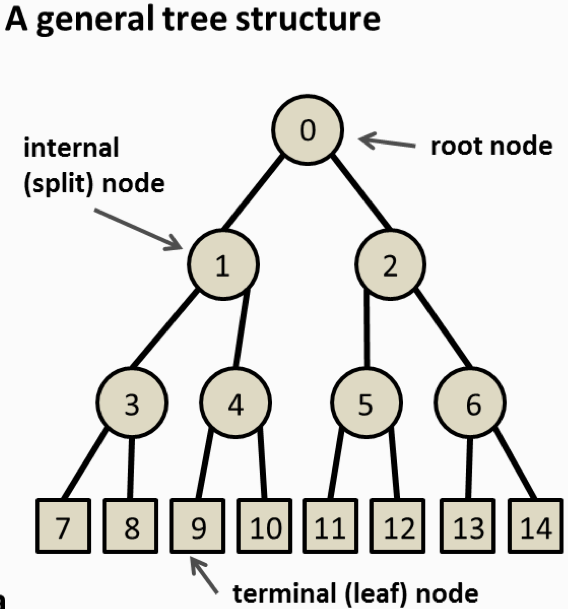
\includegraphics[height=0.7\textheight]{figures/generalTreeStructure}
% \end{center}
% \note<.>{Explain depth of a tree.}
% \end{column}
% \begin{column}{0.5\textwidth}
%     \begin{itemize}[<+->]
% \item We focus on \emph{binary} trees (as opposed to multiway trees where nodes can have more
% than two children)
% \item Each node contains a subset of data points
% \item The data splits created by each node involve only a \emph{single} feature
% \item For continuous variables, the splits are always of the form $x_{i}\le t$
% \item For discrete variables, we partition values into two sets (not covered today)
% \item Predictions are made in terminal nodes
% \end{itemize}
% \end{column}
% \end{columns}
% \let\thefootnote\relax\footnotetext{\tiny{From Criminisi et al. MSR-TR-2011-114, 28 October 2011.}}

% \note[item]{Let's review some terminology for trees you've probably seen in an algorithm class. We'll consider a rooted tree, where we have a designated root node. The nodes that have degree one (incident to only one edge) are terminal/leaf nodes. The other nodes are called internal nodes.}
% \note[item]{Specifically, we'll consider binary trees where each node has two children.}
% \note[item]{What does each node represent? They correspond to one partition of the data. The root node contains all data; we partition the data in one node by branching to its descendants.}
% \note[item]{The branching decision at each node involves a single feature.}
% \end{frame}

   
% \begin{frame}
%     {Constructing the tree}
% \begin{description}[<+->]
%         \item[Goal] Find boxes $R_1, \ldots, R_J$ that minimize $\sum\limits_{j=1}^{J}\sum\limits_{i\in R_j} (y_i - \hat y_{R_j})^2$, subject to complexity constraints.
% \item[Problem] Finding the optimal binary tree is computationally intractable.
% \item[Solution] Greedy algorithm: starting from the root, and repeating until a stopping criterion is reached (\eg max depth), find the non-terminal node that results in the ``best'' split
%     \begin{itemize}
%         \item We only split regions defined by previous non-terminal nodes
%     \end{itemize}
% \item[Prediction] Our prediction is the mean value of a terminal node: $\hat y_{R_m} = \text{mean}(y_i \mid x_i \in R_m)$
%     \begin{itemize}
% \item A greedy algorithm is the one that make the best \textbf{local} decisions, without lookahead to evaluate their downstream consequences
%     \item This procedure is not very likely to result in the globally optimal tree
%     \end{itemize}
% \end{description}
% \note[item]{Given some stopping criteria, the next question is how do we find the split that will minimize our task loss in the end.}
% \note[item]{In general, this is intractable.}
% \note[item]{However, we can use a greedy algorithm to split each node in a locally optimal way, starting from the root.}
% \end{frame}


% \begin{frame}{Prediction in a Regression Tree}
%     \begin{minipage}{0.3\textwidth}
%         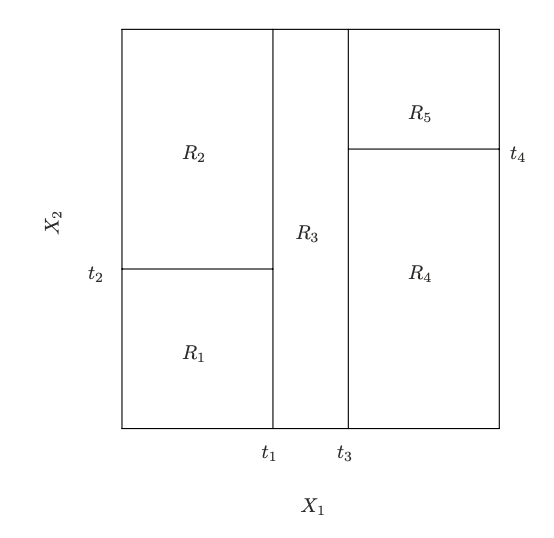
\includegraphics[height=0.5\textheight]{figures/regression_regions}
%     \end{minipage}
%     \begin{minipage}{0.6\textwidth}
%     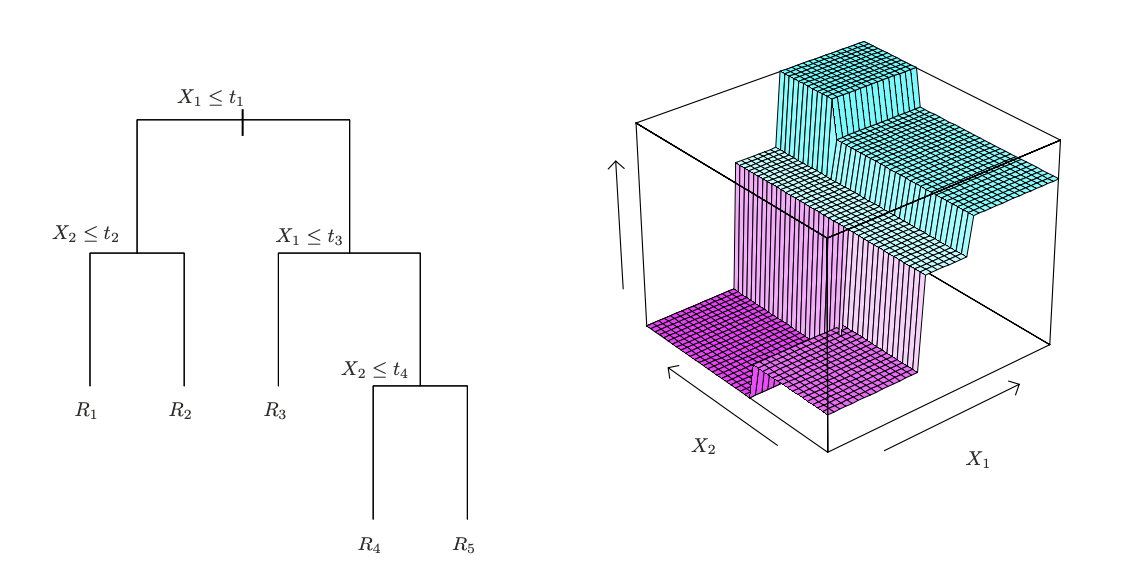
\includegraphics[height=0.6\textheight]{figures/regression_splits_and_surface}
%     \end{minipage}
% \end{frame}

% \begin{frame}{Finding the Best Split Point}
% \begin{itemize}[<+->]
% \item We enumerate all features and all possible split points for each feature. There are infinitely many split points, but...
% \item Suppose we are now considering splitting on the $j$-th feature $x_{j}$, and let $x_{j(1)},\ldots,x_{j(n)}$ be the sorted values of the $j$-th
% feature.
% \item We only need to consider split points between two adjacent values, and any split point in the interval $(x_{j(r)}, x_{(j(r+1)})$ will result in the same loss 
% \item It is common to split half way between two adjacent values:
% \begin{align}
% s_{j}\in\left\{ \frac{1}{2}\left(x_{j(r)}+x_{j(r+1)}\right)\mid r=1,\ldots,n-1\right\} .
% && \text{$n-1$ splits}
% \end{align}
% \end{itemize}

% \note[item]{Now that we have a measure of goodness for each split. How do we find that split? There are infinitely many split points for each continuous feature.}
% \note[item]{But many split points will result in the same regions.}
% \end{frame}

% \begin{frame}
%     {Decision Trees and Overfitting}
% \begin{itemize}[<+->]
% \item What will happen if we keep splitting the data into more and more regions?
% \begin{itemize}
% \item Every data point will be in its own region---\textcolor{red}{overfitting}.
% \end{itemize}

% \item When should we stop splitting? (Controlling the complexity of the hypothesis space)
% \begin{itemize}
% \item Limit total number of nodes.
% \item Limit number of terminal nodes.
% \item Limit tree depth.
% \item Require minimum number of data points in a terminal node.
% \pause
% \item \textbf{Backward pruning} (the approach used in \textbf{CART}; Breiman et al 1984): 
% \begin{enumerate}
% \item Build a really big tree (e.g. until all regions have $\le5$ points).
% \item \emph{Prune} the tree back greedily, potentially all the way to the root,
% until validation performance starts decreasing.
% \end{enumerate}
% \end{itemize}
% \end{itemize}
% \note[item]{A common approach in practice is backward pruning, similar to backward feature selection. The advantage is that we get the global view once the entire tree is built, where as in the other approaches we might stop too early and miss an important split that only comes later.}
% \end{frame}

% \begin{frame}{Pruning: Example}
%     \centering
%     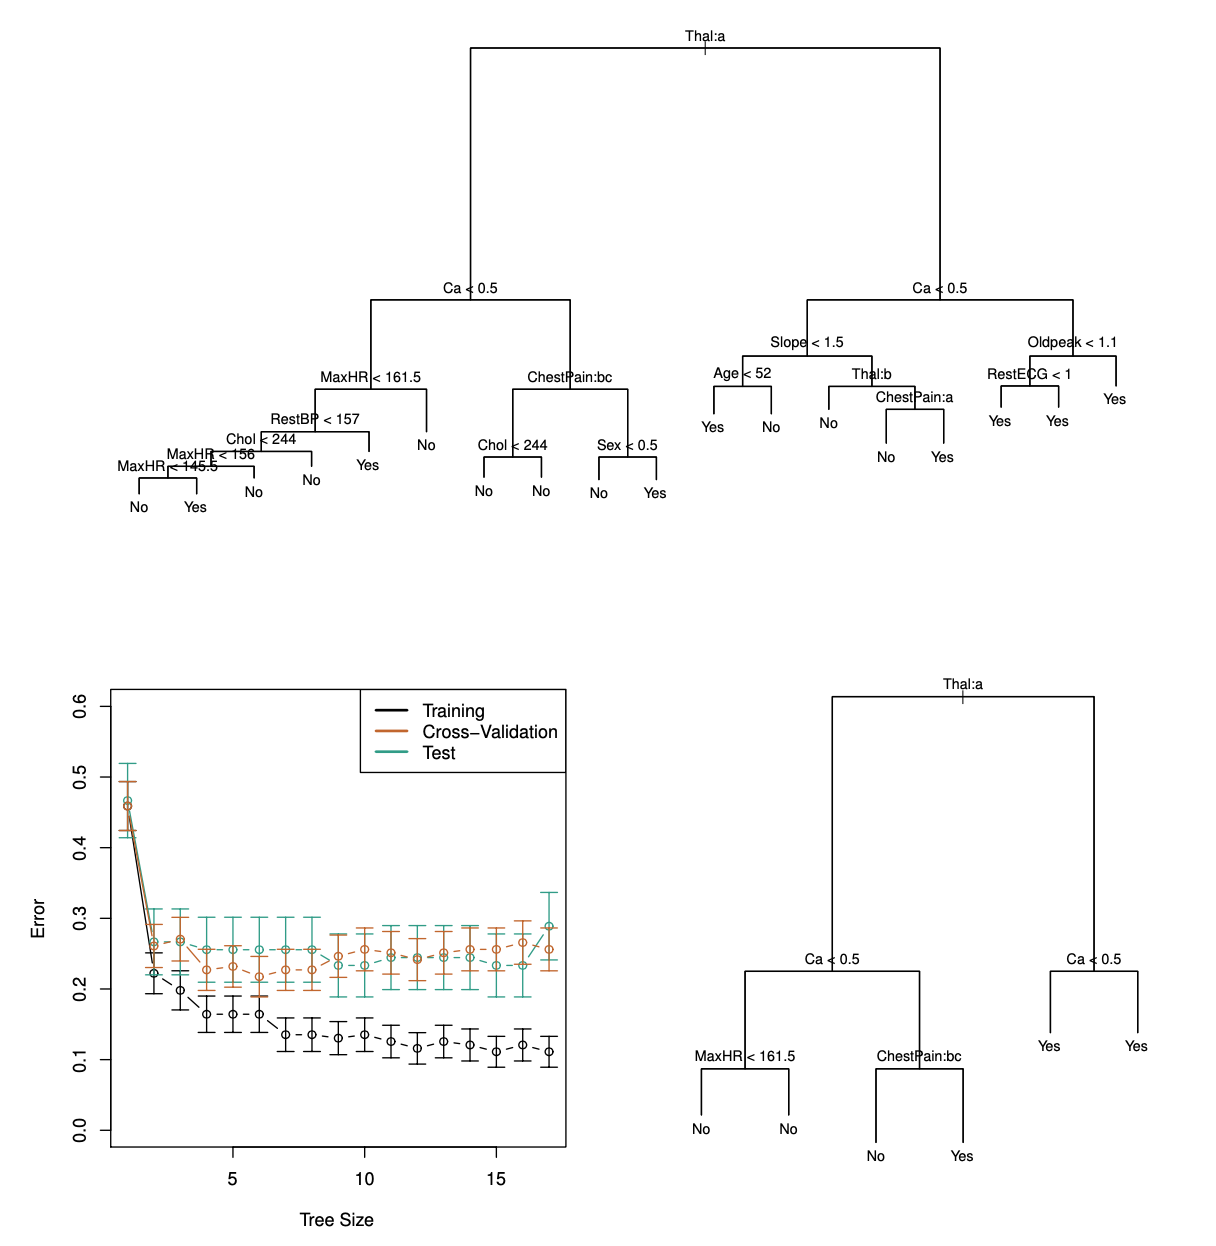
\includegraphics[height=0.8\textheight]{figures/pruning}
% \end{frame}

% \begin{frame}
% {What Makes a Good Split for Classification?}

% Our plan is to predict the \textbf{majority label} in each region.
% \onslide<+->{
%     \begin{simpleblock}{Which of the following splits is better?}
% \begin{description}
% \item[Split 1] $R_1: 8+ / 2- \qquad R_2: 2+ / 8-$
% \item[Split 2] $R_1: 6+ / 4- \qquad R_2: 4+ / 6-$
% \end{description}
% \end{simpleblock}
% }
% \onslide<+->{
%     \begin{simpleblock}{How about here?}
% \begin{description}
% \item[Split 1] $R_1: 8+ / 2- \qquad R_2: 2+ / 8-$
% \item[Split 2] $R_1: 6+ / 4- \qquad R_2: 0+ / 10-$
% \end{description}
% \end{simpleblock}
% }

% \onslide<+->{
% Intuition: we want to produce \emph{pure} nodes,
% \ie nodes where most instances have the same class.
% }
% \note[item]{Split 1 is better because it has low error rate.}
% \note[item]{It's a bit tricky now. Both split has the same error rate. Note that in Split 2, R2 would be a terminal node already, so we might prefer Split 2; however, R1 still needs more work.}
% \end{frame}

% \begin{frame}
% {Misclassification error in a node}
% \begin{itemize}
% \item Let's consider the multiclass classification case: $\cy=\left\{ 1,2,\ldots,K\right\} $.

% \item Let node $m$ represent region $R_{m}$, with $N_{m}$ observations
% \pause
% \item We denote the proportion of observations in $R_{m}$ with class $k$ by
% \[
% \hat{p}_{mk}=\frac{1}{N_{m}}\sum_{\left\{ i:x_{i}\in R_{m}\right\} }\ind{y_{i}=k}.
% \]
% \pause
% \item We predict the majority class in node $m$: 
%     \[ 
%         k(m)=\argmax_{k}\hat{p}_{mk} 
%     \]

% %\item The misclassification rate in node $m$ is $1-\hat{p}_{mk(m)}$
% \end{itemize}

% \note[item]{Each node contains a subset of data.}
% \end{frame}

% \begin{frame}{Node Impurity Measures}
% \begin{itemize}[<+->]
% \item Three measures of \textbf{node impurity} for leaf node
% $m$:
% \begin{itemize}[<+->]
% \item Misclassification error
% \[
% 1 -  \hat{p}_{mk(m)}.
% \]

% \item The Gini index encourages $\hat{p}_{mk}$ to be close to 0 or 1
% \[
% \sum_{k=1}^{K}\hat{p}_{mk}(1-\hat{p}_{mk}).
% \]

% \item Entropy / Information gain
% \[
% -\sum_{k=1}^{K}\hat{p}_{mk}\log\hat{p}_{mk}.
% \]
% \end{itemize}
% \item The Gini index and entropy are numerically similar to each other, and both work better in practice than the misclassification error.

% \note[item]{We would like a metric that gives high scores to nodes containing examples from many different classes, and low scores to nodes with few or a single class of examples.}
% \note[item]{We've seen that the error rate can indicate node purity. When is it minimized? When $p$ is 1, i.e., all examples are in the same class. Note that this is different from the Gini index that measure inequality you might learn in economics.}
% \note[item]{But it's not a ``sensitive'' measure. It's often the case that we will have many splits that gives the same misclassification error. Gini index is another popular metric. For each class $k$ we compute the product of the proportion of class $k$, $\hat{p}_{mk}$ and the other classes $1-\hat{p}_{mk}$. When is it minimized? $p=0 / 1$.}
% \note[item]{Finally, we can use Shannon entropy, which measure the uncertainty of the label in this node. It's minimized when all labels are the same---no uncertainty.}
% \note[item]{Both Gini index and entropy are information-theoretic measures.}

% \end{itemize}
% \end{frame}

% \begin{frame}{Impurity Measures for Binary Classification}

%     \centering
%     ($p$ is the relative frequency of class 1)
% \begin{figure}
% 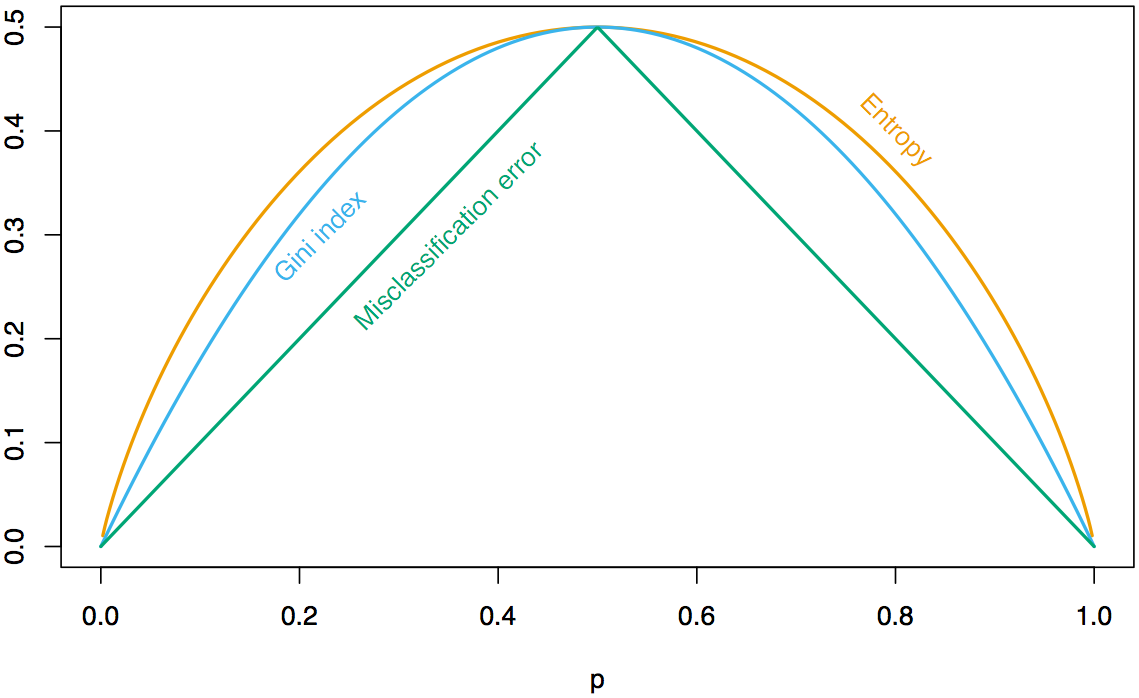
\includegraphics[height=0.5\textheight]{figures/impurityMeasureTwoClass}
% \end{figure}
% \vspace{-1em}
% %Misclassification error is not strictly concave thus may not guarantee improvement over the parent node.
% \note[item]{On the linear piece of misclassification error,
% $w_1Q(p_1) + w_2Q(p_2) = Q(w_1p_1 + w_2p_2)$.}
% \let\thefootnote\relax\footnotetext{\tiny{HTF Figure 9.3}}
% \end{frame}

% \begin{frame}{Quantifying the Impurity of a Split}
% Scoring a potential split that produces the nodes $R_{L}$ and $R_{R}$:
% \begin{itemize}
% \item Suppose we have $N_{L}$ points in $R_{L}$ and $N_{R}$ points in
% $R_{R}$.
% \pause

% \item Let $Q(R_{L})$ and $Q(R_{R})$ be the node impurity measures for each node.
% \pause

% \item We aim to find a split that minimizes the \emph{weighted average of node
% impurities}:
% \[
% \frac{N_{L}Q(R_{L})+N_{R}Q(R_{R})}{N_L+N_R}
% \]
% \end{itemize}

% \note[item]{Now that we've defined impurity measure for a single node, how do we use it to evaluate a split, which produces two nodes?}
% \note[item]{The weight is just the proportion of examples in left and right nodes.}
% \note[item]{$Q_1 = 1/4, Q_2=1/4, w_1 = 10/15=2/3, w_2 = 1/3.$}
% \end{frame}

% % \begin{frame}
% % {Regression trees}
% % \begin{itemize}
% % \item Squared loss as the node impurity measure.
% % %\item Everything else remains the same as classification trees.
% % \end{itemize}

% % \note[item]{How do we apply the same splitting strategy for regression problems? What needs to be changed?}
% % \note[item]{First, instead of predicting the majority class, we predict the mean.}
% % \note[item]{Impurity is easier---just squared loss, i.e. how much the values deviate from the mean.}
% % \note[item]{So, to recap, to grow a basic decision tree, we pick an impurity measure and a stopping criterion, start from the root node, then recursively split until a stop criteria is reached. Next, let's consider some practical matters.}
% % \end{frame}

% %\subsection{Trees in General}
% %\begin{frame}
% %{\dis Categorical features}
% %\begin{itemize}[<+->]
% %\item For a categorical feature, we split its values into two groups.
% %\item<.-> Given a set of categories of size $k$, how many distinct splits? (its power set)
% %\item Finding the optimal split is \textcolor{red}{intractable} in general.
% %\item Approximations
% %\begin{description}[<.->][Numeric encoding]
% %\item<+->[Numeric encoding] Randomly assign a number to each category
% %\begin{itemize}
% %\item Binary classification: proportion of class 0
% %\item Regression: mean of targets of examples in the category, \ie  \textbf{mean encoding} 
% %\end{itemize}
% %\item[One-hot encoding] May grow imbalanced trees, \eg left-branching
% %\item[Binary encoding] Robust to large cardinality
% %\end{description}

% %\item Statistical issues with categorical features
% %\begin{itemize}[<.->]
% %\item If a category has a very large number of categories, we can \al{overfit}.
% %\item Extreme example: Row Number could lead to perfect classification with
% %a single split.
% %\end{itemize}
% %\end{itemize}
% %\note[item]{One unique characteristic of tree-based models is that they handle categorical features naturally.}
% %\note[item]{$2^k$ subsets, divided by 2 for symmetry, minus 1 to remove the empty set}
% %\note[item]{Approximation: we can either reduce it to the continuous case, or reduce the number of categories.
% %To reduce it to the continuous case, we can randomly assign a number to each category. In binary classification, we can do it slightly smartly by assigning the proportion of negative examples in that category.
% %To reduce the number of categories, we can use binary encoding, which creates multiple binary features out of one categorical features.}
% %\note[item]{We should be careful with overfitting with there are a large number of categories though.}
% %\end{frame}

% \begin{frame}
% {Discussion: Interpretability of Decision Trees}

%     \centering
%         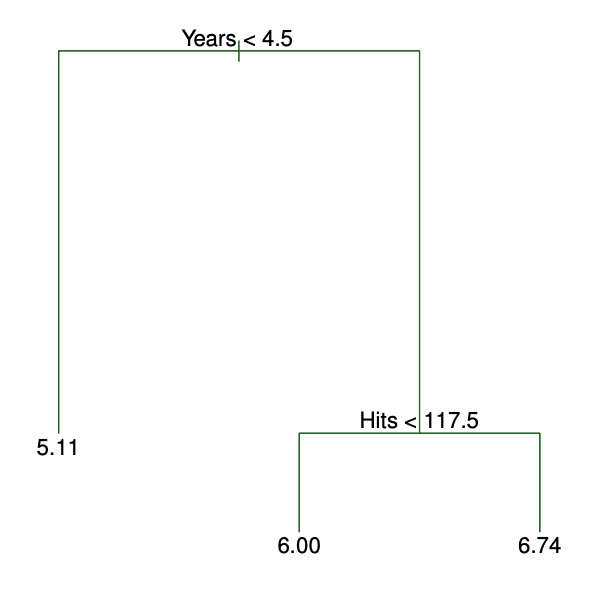
\includegraphics[width=0.2\textwidth]{figures/basketball_decision_tree}
%     \begin{itemize}[<+->]
%     \item Trees are easier to visualize and explain than other classifiers (even linear regression)
% \item Small trees are interpretable -- large trees, maybe not so much
% %\item Approximate neural network decision boundaries to gain interpretability
% %\begin{itemize}
% %\item Wu M, Hughes M, Parbhoo S, Zazzi M, Roth V, Doshi-Velez F. \href{https://finale.seas.harvard.edu/files/finale/files/beyond_sparcity_tree_regularization_of_deep_01.pdf}{Beyond Sparsity: Tree Regularization of Deep Models for Interpretability}. Association for the Advancement of Artificial Intelligence (AAAI). 2018
% %\end{itemize}
% \end{itemize}
% \end{frame}

% \begin{frame}
% {Discussion: Trees vs. Linear Models}
% Trees may have to work hard to capture linear decision boundaries, but can easily capture certain nonlinear ones:
% \begin{figure}
% 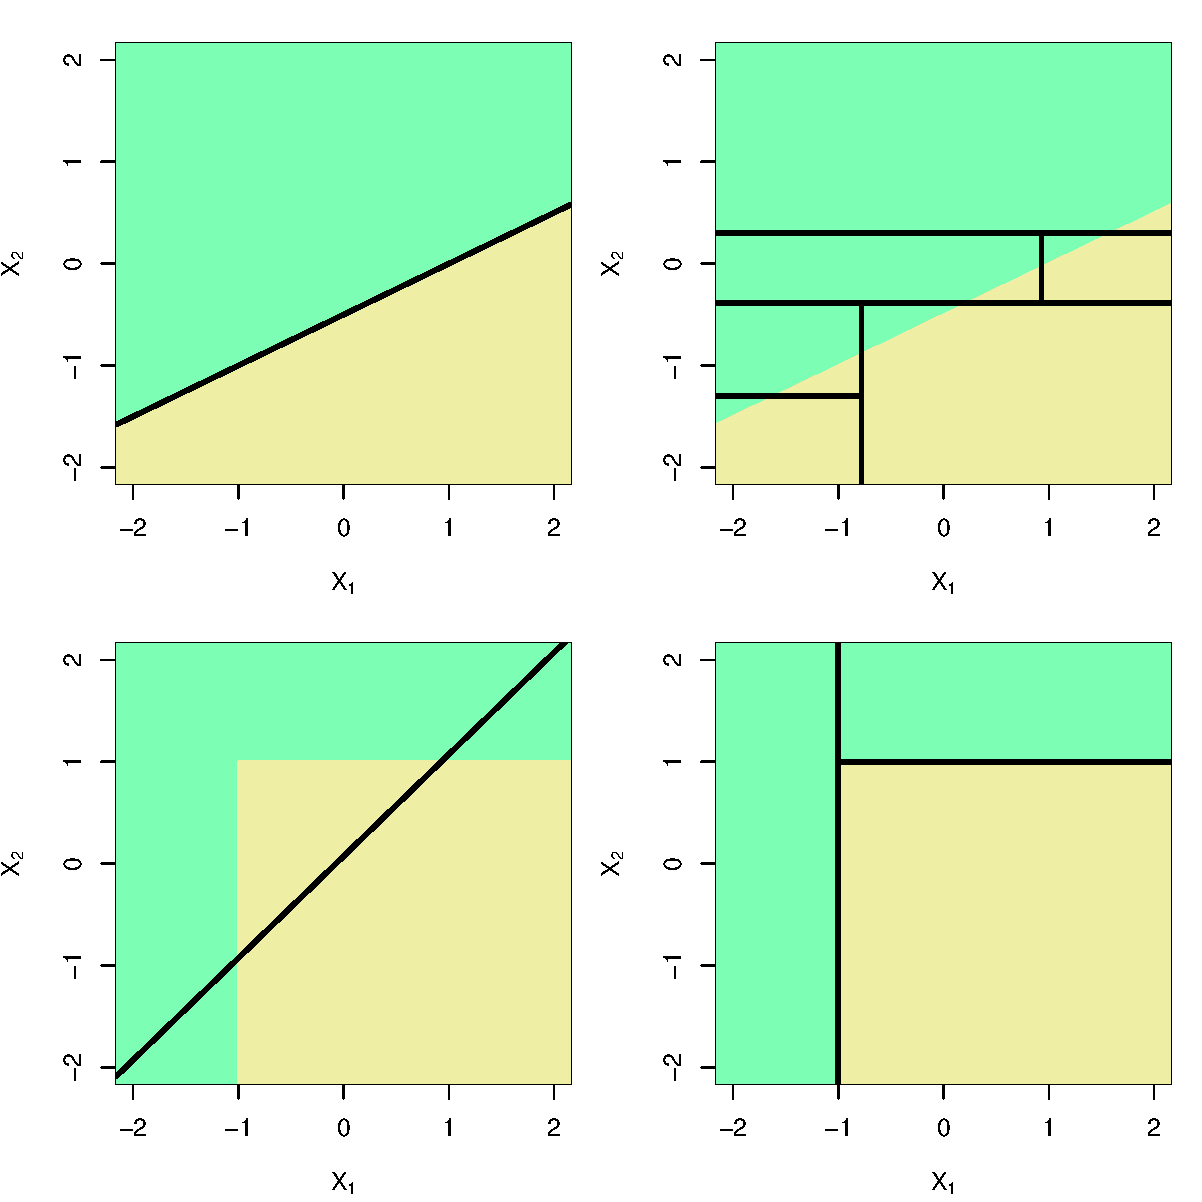
\includegraphics[height=0.6\textheight]{figures/treeVsLinear}
% \end{figure}
% \note[item]{Because it's hard of it to model the addition of two features.}
% \end{frame}

% \begin{frame}
% {Discussion: Review}
% \begin{simpleblock}{Decision trees are:}
% \begin{itemize}
% \item Non-linear: the decision boundary that results from splitting may end up being quite complicated
% \item Non-metric: they do not rely on the geometry of the space (inner products or distances)
% \item Non-parametric: they make no assumptions about the distribution of the data
% \end{itemize}
% \end{simpleblock}

% \pause
% \begin{simpleblock}{Additional pros:}
% \begin{itemize}
% \item Interpretable and simple to understand
% \end{itemize}
% \end{simpleblock}

% \pause
% \begin{simpleblock}{Cons:}
% \begin{itemize}
% \item Struggle to capture linear decision boundaries
% \item They have high variance and tend to \al{overfit}: they are sensitive to small changes in the training data (The ensemble techniques we discuss next can mitigate these issues)
% \end{itemize}
% \end{simpleblock}

% \note[item]{What are some pros and cons of trees?}
% \note[item]{One big issue with trees is that they are very unstable, meaning that if the training data is changed slightly, our classifier will be quite different, and this makes the performance of a single tree not competitive.}
% \end{frame}

\begin{frame}{Review: Decision Trees}
\begin{itemize}
\item Non-linear, non-metric, and non-parametric.
\item Regression or classification.
\pause
\item Interpretable, up to certain depth.
\pause
\item Greedy algorithm -- maximizing the purity of nodes.
\pause
\item Can overfit -- need to limit the capacity.
\end{itemize}
\end{frame}

\section{Bagging and Random Forests}
\subsection{Variance of an Estimator}
\begin{frame}
{Recap: Statistics and Point Estimators}
    \begin{itemize}[<+->]
\item We observe data $\cd=\left(x_{1},x_{2},\ldots,x_{n}\right)$ sampled i.i.d. from a parametric distribution $p(\cdot\mid \theta)$

\item A \textbf{statistic} $s=s(\cd)$ is any function of the data:
\begin{itemize}
\item E.g., sample mean, sample variance, histogram, empirical data distribution
\end{itemize}

\item A statistic $\hat{\theta}=\hat{\theta}(\cd)$ is a \textbf{point estimator}
of $\theta$ if $\hat{\theta}\approx\theta$
\end{itemize}

%\onslide<+->{
%\begin{block}{Review questions}
%In frequentist statistics,
%\begin{itemize}
%\item Is $\theta$ random?
%\item Is $\hat{\theta}$ random?
%\item Is the function $s(\cdot)$ random?
%\end{itemize}
%\end{block}
%}

\note[item]{When we say trees are not stable or have high variance, what do we mean by that precisely? Let's recall properties of point estimators we talked about in frequentist statistics.}
\note[item]{We call a statistic a point estimator if it approximates some unknown parameter.}
\note[item]{The function $s$ is not random, but we plug in random samples of data.}
\end{frame}

\begin{frame}
{Recap: Bias and Variance of an Estimator}
\begin{itemize}[<.->]
    \setlength\itemsep{2pt}
\item Statistics are random, so they have probability distributions.
\item The distribution of a statistic is called a \textbf{sampling distribution}. 
\item<+-> The standard deviation of the sampling distribution is called the \textbf{standard error}.
\item<+-> Some parameters of the sampling distribution we might be interested in:
\begin{description}
\item[Bias]  $\mbox{Bias}(\hat{\theta})\eqdef \ex\pb{\hat{\theta}}-\theta$.
\item[Variance] $\mbox{Var}(\hat{\theta})\eqdef \ex\pb{\hat{\theta}^{2}} - \ex^2\pb{\hat{\theta}}$.
\end{description}
%\item<+-> \dis Is bias and variance random?
%\begin{itemize}
    \note[item]{Neither bias nor variance depend on a specific sample $\cd_{n}$.
        We are \emph{taking expectation over $\cd$.}}
%\end{itemize}
\item<+-> Why does variance matter if an estimator is unbiased?
\pause
\begin{itemize}
    \item {$\hat{\theta}(\sD) = x_1$ is an unbiased estimator of the mean of a Gaussian, but would be farther away from $\theta$ than the sample mean.}
\end{itemize}
\end{itemize}
\note[item]{Next let's look at how we can reduce variance of an estimator.}
\end{frame}

\subsection{The Benefits of Averaging}
\begin{frame}
{Variance of a Mean}
\begin{itemize}
\item Let $\hat{\theta}(\sD)$ be an unbiased estimator with variance $\sigma^2$:
$\BE\pb{\hat{\theta}} = \theta$, $\mbox{Var}(\hat{\theta}) = \sigma^2$.
\item<+-> So far we have used a single statistic $\hat{\theta} = \hat{\theta}(\sD)$ to estimate $\theta$.
\item<+-> Its standard error is $\sqrt{\mbox{Var}(\hat{\theta})} = \sigma$
\end{itemize}

\onslide<+->{
\begin{itemize}
\item Consider a new estimator that takes the average of i.i.d. $\hat{\theta}_1, \ldots, \hat{\theta}_n$ where $\hat{\theta}_i = \hat{\theta}(\sD^{i})$.
    \pause
\item The average has the same expected value but smaller standard error (recall that $Var(cX) = c^2 Var(X)$, and that the $\hat{\theta}_i$-s are uncorrelated):
\begin{align}
\BE\pb{\frac{1}{n}\sum_{i=1}^n \hat{\theta}_i} = \theta \qquad
\mbox{Var}\pb{\frac{1}{n}\sum_{i=1}^n \hat{\theta}_i} = \frac{\sigma^2}{n}
\label{eqn:variance-of-sample-mean}
\end{align}
\end{itemize}
}
\note[item]{Let's say we want to estimate some parameter $\theta$.}
\note[item]{What is the standard error?}
\note[item]{Now let's consider a new estimator that takes the average of $n$ i.i.d. estimates, each computed from some data $\sD^i$.}
\note[item]{It will still be unbiased, but now the variance is reduced. Try to prove it yourself.}
\end{frame}

\begin{frame}{Averaging Independent Prediction Functions }
    \begin{itemize}[<+->]
\item Suppose we have $B$ independent training sets, all drawn from the same distribution ($\sD \sim p(\cdot\mid \theta)$).

\item Our learning algorithm gives us $B$ prediction functions: $\hat{f}_{1}(x),\hat{f}_{2}(x),\ldots,\hat{f}_{B}(x)$

\item We will define the average prediction function as:
\begin{align}
\hat{f}_{\text{avg}}\eqdef \frac{1}{B}\sum_{b=1}^{B}\hat{f}_{b}
\end{align}

%\item<+-> \dis What's random here?
%\begin{itemize}
    \note[item]{The $B$ independent training sets are random, which gives rise to
        variation among the $\hat{f}_{b}$'s.}
%\end{itemize}

%\item<+-> \think{Concept check}: What's the distribution of $\hat{f}$ called?
%What do we know about the distribution?
\end{itemize}

\note[item]{Concept check: sampling distribution. We don't know anything about it because we don't know the data generating distribution.}
\end{frame}

%
\begin{frame}{Averaging Reduces Variance of Predictions}
\begin{itemize}
\item The average prediction for $x_{0}$ is
\[
\hat{f}_{\text{avg}}(x_{0})=\frac{1}{B}\sum_{b=1}^{B}\hat{f}_{b}(x_{0}).
\]

\item $\hat{f}_{\text{avg}}(x_{0})$ and $\hat{f}_{b}(x_{0})$ have the
same expected value, but

\item $\hat{f}_{\text{avg}}(x_{0})$ has smaller variance:% (see \ref{eqn:variance-of-sample-mean}):
\begin{eqnarray*}
\mbox{\ensuremath{\var}}(\hat{f}_{\mbox{avg}}(x_{0})) = 
\frac{1}{B}\var\left(\hat{f}_{1}(x_{0})\right)
\end{eqnarray*}
\pause
\item \al{Problem}: in practice we don't have $B$ independent training sets!
\end{itemize}
\note[item]{The average prediction has the same expected value as the single prediction, but it has smaller variance.}
\note[item]{But are we done? Just train $n$ predictors and average them?}
\end{frame}

\subsection{Bootstrap}

\begin{frame}{The Bootstrap Sample}
\begin{simpleblock}
{How do we simulate multiple samples when we only have one?}
\begin{itemize}[<+->]
\item A \textbf{bootstrap sample} from $\cd_{n}=\left(x_{1},\ldots,x_{n}\right)$
is a sample of size $n$ drawn \emph{with replacement} from $\cd_{n}$

\item Some elements of $\cd_{n}$ 
will show up multiple times, and
some won't show up at all 
\end{itemize}
\end{simpleblock}

%\onslide<+->{\dis How similar are the bootstrap samples?}
\begin{itemize}[<+->]
\item Each $x_{i}$ has a probability of $(1-1/n)^{n}$ of not being
included in a given bootstrap sample

\item For large $n$,
\begin{align}
\left(1-\frac{1}{n}\right)^{n}\approx\frac{1}{e}\approx.368.
\end{align}

\item<.-> So we expect \textasciitilde 63.2\% of elements of $\cd_n$ will show
up at least once.
\end{itemize}

\note[item]{Now the question is how similar these bootstrap samples are. If they are pretty much the same, its distribution would be far from the actual data generating distribution.}
\note[item]{Because we are sampling with replacement, each element has $1/n$ probability to be selected during each draw. And after $n$ draws, the probability that it's still not selected is $1-1/n$ to the power of $n$.}
\note[item]{Actually $n$ doesn't have to be very large, with $n=1000$, we already reach this number here.}
\note[item]{Since about 60 percent examples shown in each bootstrap sample, they should be fairly different.}
\end{frame}
%
%
\begin{frame}{The Bootstrap Method}
\begin{definition}
A \textbf{bootstrap method } simulates $B$
independent samples from $P$ by taking $B$ bootstrap samples from
the sample $\cd_{n}$.

\end{definition}
\pause

\begin{itemize}
\item Given original data $\cd_{n}$, compute $B$ bootstrap samples $D_{n}^{1},\ldots,D_{n}^{B}$.

\pause
\item For each bootstrap sample, compute some function
\[
\phi(D_{n}^{1}),\ldots,\phi(D_{n}^{B})
\]
\pause

\item Use these values as though $D_{n}^{1},\ldots,D_{n}^{B}$ were
i.i.d. samples from $P$.

\item This often ends up being very close to what we'd get with independent samples from $P$!
\end{itemize}
\end{frame}
%
\begin{frame}{Independent Samples vs. Bootstrap Samples}
\begin{itemize}
\item Point estimator $\hat{\alpha}=\hat{\alpha}(\cd_{100})$ for samples
of size $100$, for a synthetic case where the data generating distribution is known

\item Histograms of $\hat{\alpha}$ based on
\begin{itemize}
    \item 1000 independent samples of size 100 (left), vs.
    \item 1000 bootstrap samples of size 100 (right)

\end{itemize}
\end{itemize}
\begin{figure}
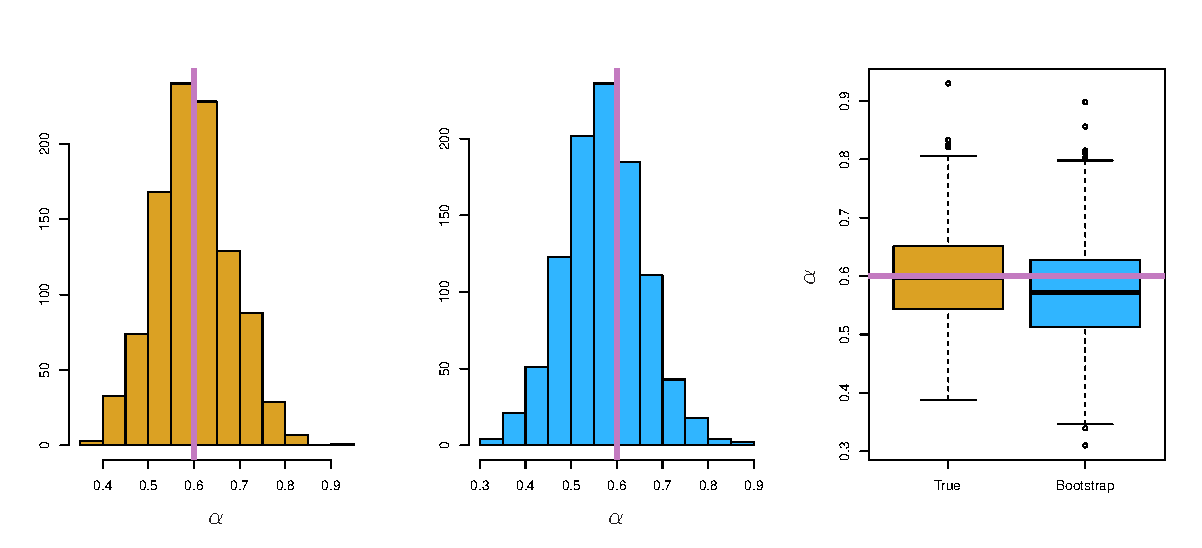
\includegraphics[height=0.4\textheight]{figures/independentVsBootstrap}

\end{figure}

\let\thefootnote\relax\footnotetext{\tiny{Figure 5.10 from \emph{ISLR} (Springer, 2013) with permission from the authors: G. James, D. Witten,  T. Hastie and R. Tibshirani.}}
\end{frame}
%
%\begin{frame}{Side note: Bootstrap in Practice}
%We can use bootstrap to get error bars in a cheap way.
%\begin{itemize}
%\item Suppose we have an estimator $\hat{\theta}=\hat{\theta}(\cd_{n})$.

%\item To get error bars, we can compute the ``\emph{bootstrap variance}''. 

%\begin{itemize}

%\item Draw $B$ bootstrap samples.
%\item Compute sample variance of $\hat{\theta}(\cd_{n}^{1}),\ldots,\hat{\theta}(\cd_{n}^{B})$..

%\item Could report 
%\[
%\hat{\theta}(\cd_{n})\pm\sqrt{\mbox{Bootstrap Variance}}
%\]

%\end{itemize}
%\end{itemize}
%\end{frame}

\begin{frame}{Ensemble Methods}

{\textbf{Key ideas:}}

    \begin{itemize}[<+->]
    \item In general, \textbf{ensemble methods} combine multiple weak models into a single, more powerful model
    \item Averaging i.i.d. estimates reduces variance without changing bias
    \item We can use bootstrap to simulate multiple data samples and average them
    \item Parallel ensemble (\eg bagging): models are built independently
    \item Sequential ensemble (\eg boosting): models are built sequentially
        \begin{itemize}
        \item We try to find new learners that do well where previous learners fall short
        \end{itemize}
\end{itemize}

\end{frame}

\subsection{Bagging}
\begin{frame}{Bagging: Bootstrap Aggregation}
    \begin{itemize}[<+->]
\item We draw $B$ bootstrap samples $D^{1},\ldots,D^{B}$ from original data
$\cd$

\item Let $\hat{f}_{1},\hat{f}_{2},\ldots,\hat{f}_{B}$ be the prediction
functions resulting from training on $D^{1},\ldots,D^{B}$, respectively

\item The \textbf{bagged prediction function} is a \emph{combination }of
these:
\[
\hat{f}_{\text{avg}}(x)=\mbox{Combine}\left(\hat{f}_{1}(x),\hat{f}_{2}(x),\ldots,\hat{f}_{B}(x)\right)
\]

%\pause{}
%\item \dis How might we combine 
%\begin{itemize}
%\item prediction functions for regression?
%\item binary class predictions? 
%\item binary probability predictions?
%\item multiclass predictions? 
%\end{itemize}

    \end{itemize}
\end{frame}

\begin{frame}{Bagging: Bootstrap Aggregation}
    \begin{itemize}[<+->]

\item Bagging is a general method for variance reduction, but it is particularly useful for decision trees

\item For classification, averaging doesn't make sense; we can take a \textbf{majority vote} instead

\item Increasing the number of trees we use in bagging does not lead to overfitting

\item Is there a downside, compared to having a single decision tree?

\item Yes: if we have many trees, the bagged predictor is much less interpretable

\end{itemize}
\end{frame}

\begin{frame}{Aside: Out-of-Bag Error Estimation}
\begin{itemize}
\item Recall that each bagged predictor was trained on about 63\% of the data.
\item The remaining 37\% are called \textbf{out-of-bag (OOB)} observations.

\pause{}
\item For $i$th training point, let 
\[
S_{i}=\left\{ b\mid D^{b}\text{ does not contain }i\text{th point}\right\} 
\]

\item The \textbf{OOB prediction} on $x_{i}$ is
\[
\hat{f}_{\text{OOB}}(x_{i})=\frac{1}{\left|S_{i}\right|}\sum_{b\in S_{i}}\hat{f}_{b}(x_{i})
\]
\pause
\item The OOB error is a good estimate of the test error

\item Similar to cross validation error: both are computed
on the training set
\end{itemize}
\end{frame}

\begin{frame}{Applying Bagging to Classification Trees}
\begin{itemize}
\item Input space $\cx=\reals^{5}$ and output space $\cy=\left\{ -1,1\right\} $.
Sample size $n=30$.
\begin{columns}[t]

\column{.4\textwidth}

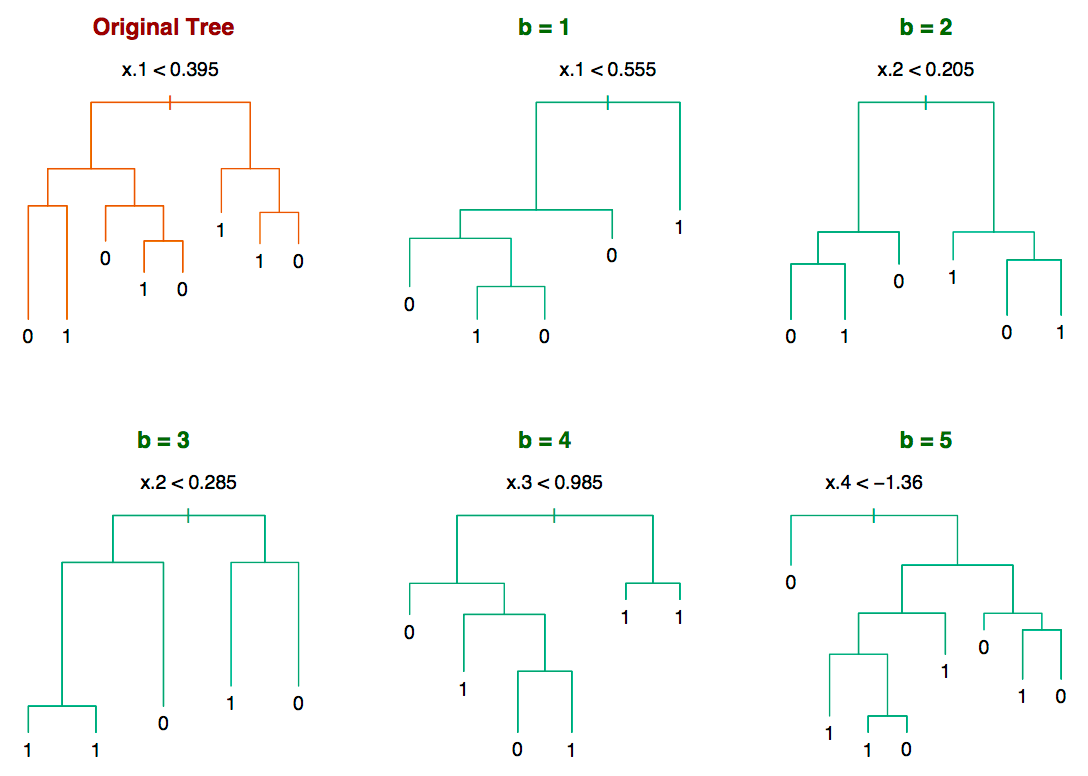
\includegraphics[width=1\columnwidth]{figures/baggedTrees}

\pause{}

\column{.6\textwidth}
\begin{itemize}[<+->]
\item Each bootstrap tree is quite different: different splitting variable at the root!

\item \textbf{High variance}: small perturbations of the training data lead to a high degree of model variability

\item Bagging helps most when the base learners are relatively unbiased but have high variance (exactly the case for
    decision trees)

\end{itemize}
\end{columns}

\end{itemize}
\let\thefootnote\relax\footnotetext{\tiny{From HTF Figure 8.9}}
\end{frame}
%

\subsection{Random Forests}
\begin{frame}{Motivating Random Forests: Correlated Prediction Functions}
Recall the motivating principle of bagging:
    \begin{itemize}[<+->]
\item For $\hat{\theta}_{1},\ldots,\hat{\theta}_{n}$ \emph{i.i.d.} with $\ex\pb{\hat{\theta}}=\theta$ and $\var\pb{\hat{\theta}}=\sigma^{2}$,
\[
\ex\left[\frac{1}{n}\sum_{i=1}^{n}\hat{\theta}_{i}\right]=\mu\qquad\var\left[\frac{1}{n}\sum_{i=1}^{n}\hat{\theta}_{i}\right]=\frac{\sigma^{2}}{n}.
\]

\item What if $\hat{\theta}$'s are correlated? 

%\item Suppose $\forall i\neq j$, $\text{Corr}(\hat{\theta}_{i},\hat{\theta}_{j})=\rho$ . Then
%\[
%\var\left[\frac{1}{n}\sum_{i=1}^{n}\hat{\theta}_{i}\right]=\rho\sigma^{2}+\frac{1-\rho}{n}\sigma^{2}.
%\]

\item For large $n$, the covariance term dominates, limiting the benefits of averaging
\item Bootstrap samples are 
\begin{itemize}
\item independent samples from the training set, but
\item \al{not} independent samples from $P_{\cx\times\cy}$
\end{itemize}

\item Can we reduce the dependence between $\hat{f}_{i}$'s?
\end{itemize}
\end{frame}

\begin{frame}{Random Forests}
\begin{simpleblock}{\textbf{Key idea}}
Use bagged decision trees, but modify the tree-growing procedure
to reduce the dependence between trees.
\end{simpleblock}

\begin{itemize}[<+->]
\item Build a collection of trees independently (in parallel), as before
\item When constructing each tree node, restrict choice of splitting
variable to a randomly chosen subset of features of size $m$
\begin{itemize}
    \item<.-> This prevents a situation where all trees are dominated by the same small number of strong features (and are therefore too similar to each other)
\end{itemize}
\item We typically choose $m\approx\sqrt{p}$, where $p$ is the number of
    features (or we can choose $m$ using cross validation)
\item If $m = p$, this is just bagging
\end{itemize}
\note[item]{When $m$ is too small, you might underfit. When $m$ is too large, it won't be effective at reducing dependence.}
\end{frame}
%
\begin{frame}{Random Forests: Effect of $m$} 
\begin{figure}
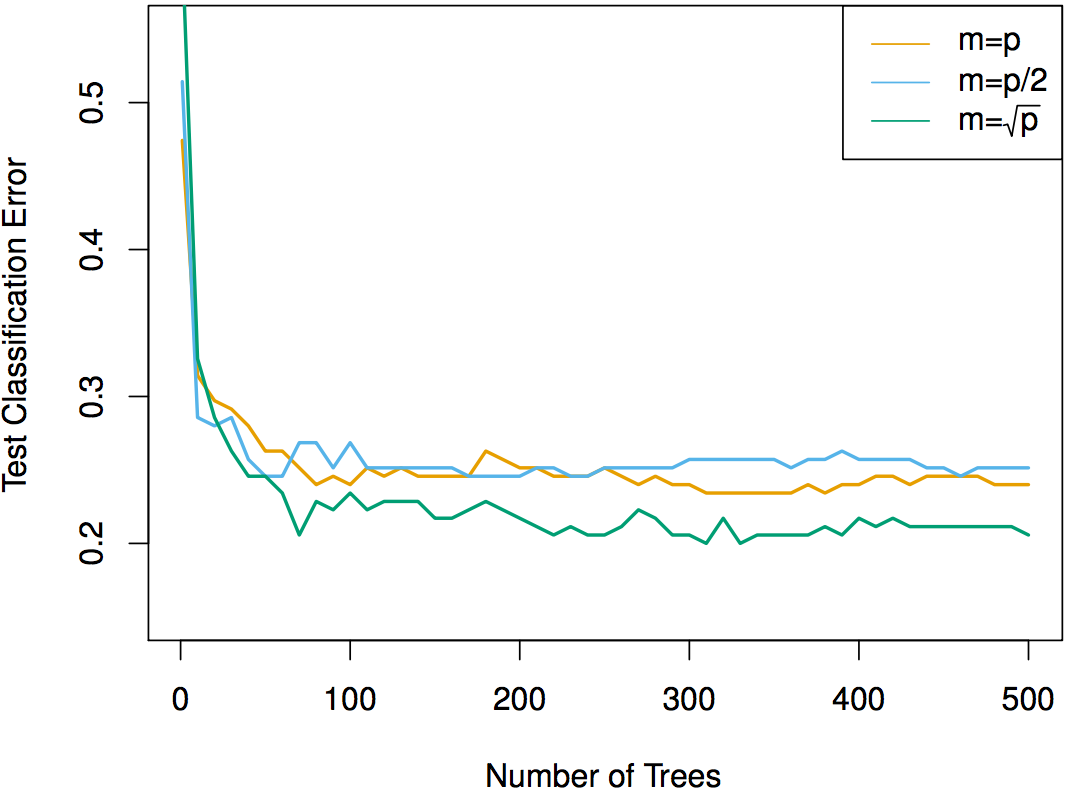
\includegraphics[height=0.7\textheight]{figures/randomForestVsBagging}
\end{figure}

\let\thefootnote\relax\footnotetext{\tiny{From \emph{An Introduction to Statistical Learning, with applications in R} (Springer, 2013) with permission from the authors: G. James, D. Witten,  T. Hastie and R. Tibshirani.}}
\end{frame}

\begin{frame}{Review}
\begin{itemize}[<+->]
\item The usual approach is to build very deep trees---low bias but \al{high variance}
\item Ensembling many models reduces variance
\begin{itemize}[<.->]
\item Motivation: Mean of i.i.d. estimates has smaller variance than single estimate
\end{itemize}
\item Use bootstrap to simulate many data samples from one dataset
\begin{itemize}[<.->]
\item $\implies$ Bagged decision trees
\end{itemize}
\item But bootstrap samples (and the induced models) are correlated
\item Ensembling works better when we combine a diverse set of
prediction functions
\begin{itemize}[<.->]
    \item $\implies$ Random forests: select a random subset of features for each decision tree
\end{itemize}
\end{itemize}
\end{frame}

\section{Boosting}
\begin{frame}
{Boosting: Overview}
\begin{description}[<+->]
    \item[Bagging] Reduce variance of a low bias, high variance estimator by ensembling many estimators trained in parallel (on different datasets obtained through sampling).
\item[Boosting] Reduce the error rate of a high bias estimator by ensembling many estimators trained in sequence (without bootstrapping).
\begin{itemize}
\item Like bagging, boosting is a general method that is particularly popular with decision trees.
\item Main intuition: instead of fitting the data very closely using a large decision tree, train gradually, using a sequence of simpler trees
\end{itemize}
\end{description}
\end{frame}

    \begin{frame}{Boosting: Overview}
        \begin{itemize}[<+->]
\item A \textbf{weak/base learner} is a classifier that does slightly better than chance.
\item<.-> Weak learners are like rules of thumb:
\begin{itemize}[<.->]
\item ``Inheritance'' $\implies$ spam
\item From a friend $\implies$ not spam
\end{itemize}
\item \textbf{Key idea}:
\begin{itemize}
\item Each weak learner focuses on different training examples (\emph{reweighted data})
\item Weak learners make different contributions to the final prediction (\emph{reweighted classifier})
\end{itemize}
        \item A set of smaller, simpler trees may improve interpretability
        \item We'll focus on a specific implementation, AdaBoost (Freund \& Schapire, 1997)
\end{itemize} 
\end{frame}

\subsection{AdaBoost: The Algorithm}
\begin{frame}{AdaBoost: Setting}

\begin{itemize}[<+->]
\item Binary classification: $\cy=\left\{ -1,1\right\} $ 

\item {Base hypothesis space} $\ch=\left\{ h:\cx\to {\color{blue}\left\{ -1,1\right\}} \right\} $. 

\item Typical base hypothesis spaces:
\begin{itemize}[<.->]
\item \textbf{Decision stumps} (tree with a single split)
\item Trees with few terminal nodes
\item Linear decision functions
\end{itemize}
\end{itemize}
\end{frame}
%
\begin{frame}{Weighted Training Set}
Each base learner is trained on weighted data.
\begin{itemize}
\item Training set $\cd=\left(\left(x_{1},y_{1}\right),\ldots,\left(x_{n},y_{n}\right)\right)$.
\item Weights $\left(w_{1},\ldots,w_{n}\right)$ associated with each example.

\pause{}
\item \textbf{Weighted empirical risk}:
\[
\hat{R}_{n}^{w}(f)\eqdef \frac{1}{W}\sum_{i=1}^{n}w_{i}\ell\left(f(x_{i}),y_{i}\right)\quad\mbox{where}\;W=\sum_{i=1}^{n}w_{i}
\]

\item Examples with larger weights affect the loss more.

\end{itemize}
\end{frame}

\begin{frame}{AdaBoost: Schematic}
\begin{center}
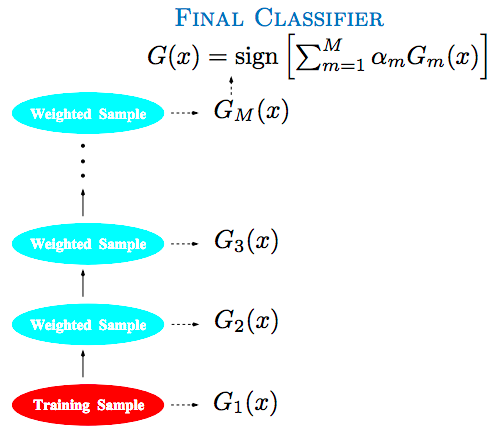
\includegraphics[height=0.7\textheight]{figures/adaboostSchematic}
\par\end{center}

\let\thefootnote\relax\footnotetext{\tiny{From ESL Figure 10.1}}
\end{frame}

\begin{frame}{AdaBoost: Sketch of the Algorithm}

\begin{itemize}[<+->]
%\item Training set $\cd=\left(\left(x_{1},y_{1}\right),\ldots,\left(x_{n},y_{n}\right)\right)$.
\item Start with equal weights for all training points: $w_{1}=\cdots=w_{n}=1$

\item Repeat for $m=1,\ldots,M$ (where $M$ is the number of classifiers we plan to train):

\begin{itemize}
\item Train base classifier $G_{m}(x)$ on the weighted training data; this classifier may not fit the data well

\item Increase the weight of the points misclassified by $G_{m}(x)$ (this is the key idea of boosting!)

\end{itemize}
%\item So far, we've generated $M$ classifiers: $G_{1},\ldots,G_{M}:\cx\to\left\{ -1,1\right\} $.
\item Our final prediction is $G(x)=\sign\left[\sum_{m=1}^{M}\alpha_{m}G_{m}(x)\right]$
\end{itemize}

\end{frame}

\begin{frame}{AdaBoost: Classifier Weights}
    \begin{itemize}
\item Our final prediction is $G(x)=\sign\left[\sum_{m=1}^{M}\alpha_{m}G_{m}(x)\right]$.
\item We would like $\alpha_{m}$ to be:
\begin{itemize}
\item Nonnegative
\item Larger when $G_{m}$ fits its weighted training data well
\end{itemize}
\item The \textbf{weighted 0-1 error} of $G_{m}(x)$ is
\[
\mbox{err}_{m}=\frac{1}{W}\sum_{i=1}^{n}w_{i}\ind{y_{i}\neq G_{m}(x_{i})}\quad\text{where }W=\sum_{i=1}^{n}w_{i}.
\]
\item $\text{err}_{m}\in[0,1]$
\end{itemize}
\end{frame}
%
\begin{frame}{AdaBoost: Classifier Weights}
\begin{itemize}
\item The weight of classifier $G_{m}(x)$ is $\alpha_{m}=\ln\left(\frac{1-\text{err}_{m}}{\text{err}_{m}}\right)$

\pause{}
\end{itemize}
\begin{center}
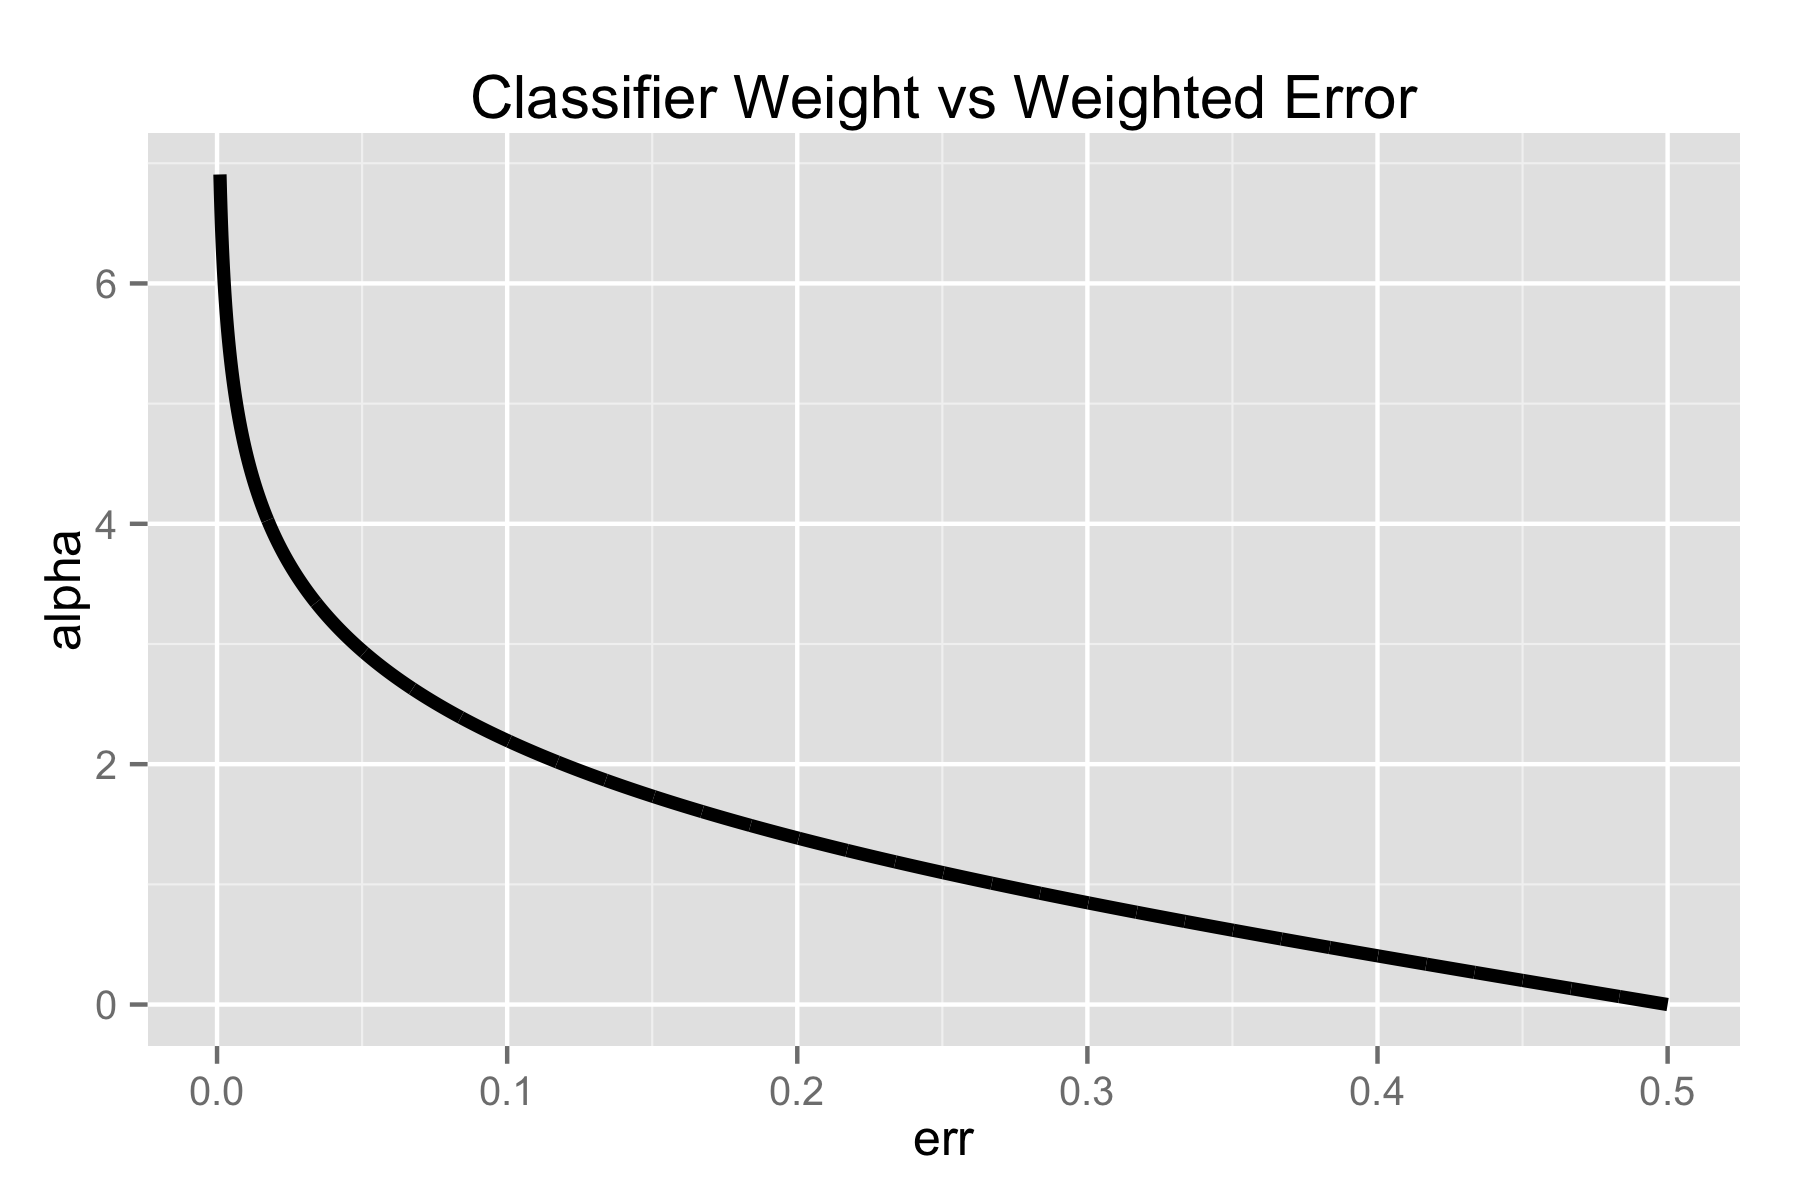
\includegraphics[clip,height=0.5\textheight]{figures/adaboostAlphaVsError}
\par\end{center}
\begin{itemize}
\item Higher weighted error $\implies$ lower weight
%\item When is $\alpha_m < 0$?
\end{itemize}

\end{frame}
%
\begin{frame}{AdaBoost: Example Reweighting}
\begin{itemize}
    \item We train $G_{m}$ to minimize weighted error; the resulting error rate is $\text{err}_{m}$

\item<.-> Then $\alpha_{m}=\ln\left(\frac{1-\text{err}_{m}}{\text{err}_{m}}\right)$
is the weight of $G_{m}$ in the final ensemble
\end{itemize}

\onslide<+->{
We want the next base learner to focus more on examples misclassified by the previous learner.
}
\begin{itemize}[<+->]
\item Suppose $w_{i}$ is the weight of example $x_i$ before training:
\begin{itemize}
\item If $G_{m}$ classifies $x_{i}$ correctly, keep $w_{i}$ as is

\item Otherwise, increase $w_{i}$:
\begin{eqnarray*}
w_{i} & \gets & w_{i}e^{\alpha_{m}}\\
& = & w_{i}\left(\frac{1-\text{err}_{m}}{\text{err}_{m}}\right)
\end{eqnarray*}

\item If $G_m$ is a strong classifier overall, then its $\alpha_m$ will be large; this means that if $x_i$ is misclassified, $w_i$ will increase to a greater extent
%\item<.-> For $\mbox{err}_{m}<0.5$ (weak learner), this always increases the weight.
\end{itemize}
\end{itemize}
\end{frame}

\begin{frame}{AdaBoost: Algorithm}

Given training set $\cd=\left\{ \left(x_{1},y_{1}\right),\ldots,\left(x_{n},y_{n}\right)\right\} $.
\begin{enumerate}
\item Initialize observation weights $w_{i}=1$, $i=1,2,\ldots,n$.

\pause{}
\item For $m=1$ to $M$:
\begin{enumerate}
\item Base learner fits weighted training data and returns $G_{m}(x)$

\pause{}
\item Compute \emph{weighted empirical 0-1 risk}:
\[
\mbox{err}_{m}=\frac{1}{W}\sum_{i=1}^{n}w_{i}\ind{y_{i}\neq G_{m}(x_{i})}\quad\text{where }W=\sum_{i=1}^{n}w_{i}.
\]
\pause{}
\item Compute  \emph{classifier weight}: $\alpha_{m}=\ln\left(\frac{1-\text{err}_{m}}{\text{err}_{m}}\right)$.

\pause{}
\item Update \emph{example weight}: $w_{i}\gets w_{i}\cdot\exp\left[\alpha_{m}\ind{y_{i}\neq G_{m}(x_{i})}\right]$

\pause{}
\end{enumerate}
\item Return \emph{voted classifier}: $G(x)=\sign\left[\sum_{m=1}^{M}\alpha_{m}G_{m}(x)\right]$.
\end{enumerate}
\end{frame}

\begin{frame}{AdaBoost with Decision Stumps}
\begin{itemize}
\item After 1 round:
\end{itemize}
\begin{figure}
\begin{centering}
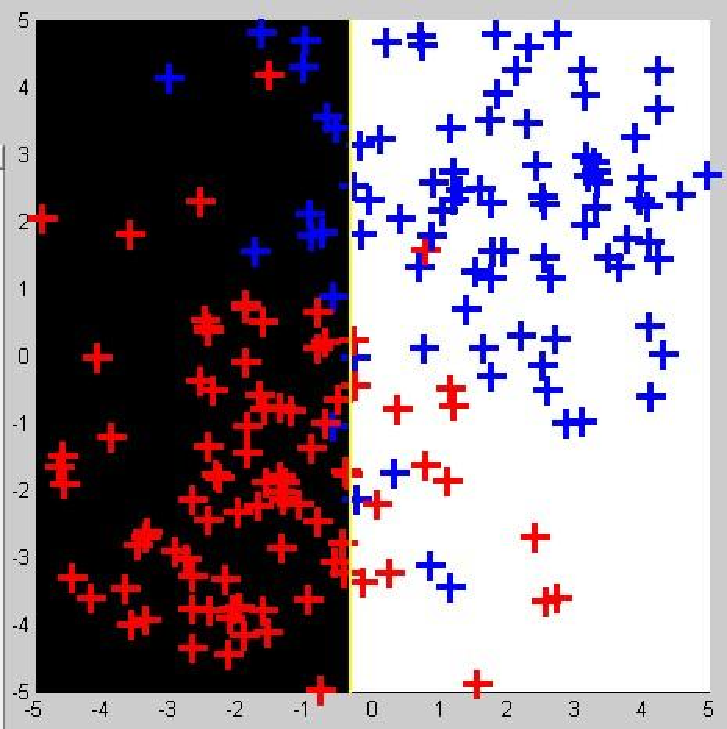
\includegraphics[height=0.5\textheight]{{figures/fig16.10a}.pdf}
\par\end{centering}
\caption{{\footnotesize{}Size of plus sign represents weight of example. Blackness represents preference for red class; whiteness represents preference for blue class.}}
\end{figure}

\let\thefootnote\relax\footnotetext{\tiny{KPM Figure 16.10}}
\end{frame}
%
\begin{frame}{AdaBoost with Decision Stumps}
\begin{itemize}
\item After 3 rounds:
\end{itemize}
\begin{figure}
\begin{centering}
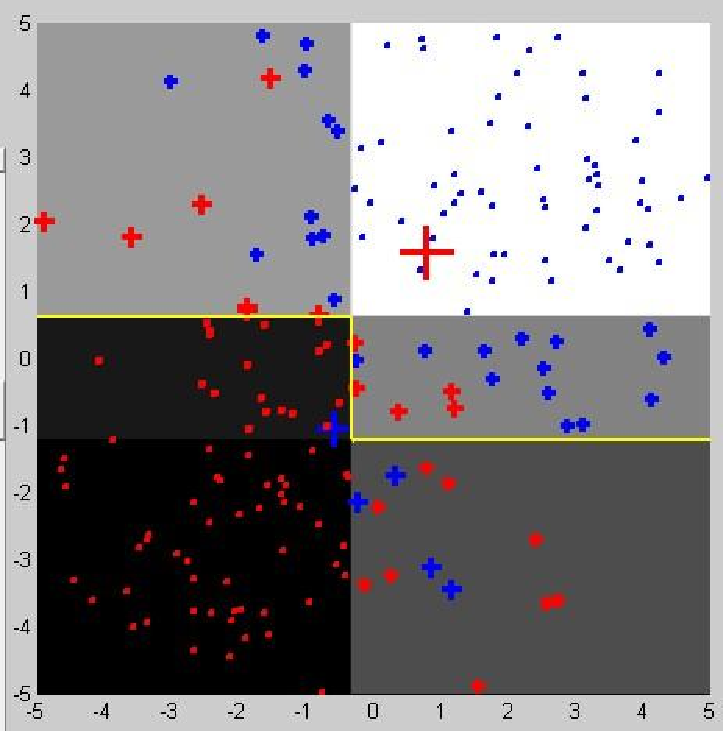
\includegraphics[clip,height=0.5\textheight]{{figures/fig16.10b}.pdf}
\par\end{centering}
\caption{{\footnotesize{}Size of plus sign represents weight of example. Blackness represents preference for red class; whiteness represents preference for blue class.}}
\end{figure}

\let\thefootnote\relax\footnotetext{\tiny{KPM Figure 16.10}}
\end{frame}
%
\begin{frame}{AdaBoost with Decision Stumps}
\begin{itemize}
\item After 120 rounds:
\end{itemize}
\begin{figure}
\begin{centering}
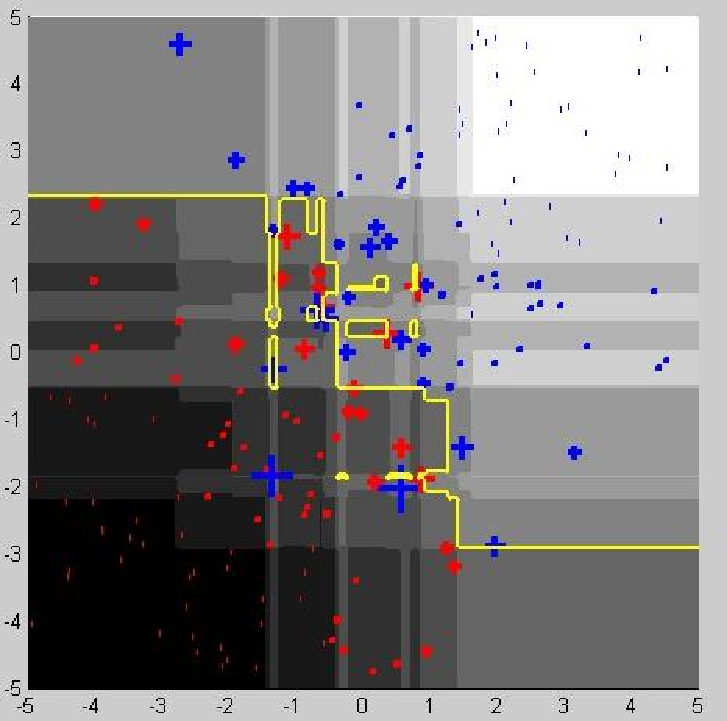
\includegraphics[height=0.5\textheight]{{figures/fig16.10c}.pdf}
\par\end{centering}
\caption{{\footnotesize{}Size of plus sign represents weight of example. Blackness represents preference for red class; whiteness represents preference for blue class.}}
\end{figure}

\let\thefootnote\relax\footnotetext{\tiny{KPM Figure 16.10}}
\end{frame}

\begin{frame}{Does AdaBoost overfit?}
\begin{itemize}
\item Does a large number of rounds of boosting lead to overfitting?
\item If we were overfitting, the learning curves would look like:
\end{itemize}
\begin{center}
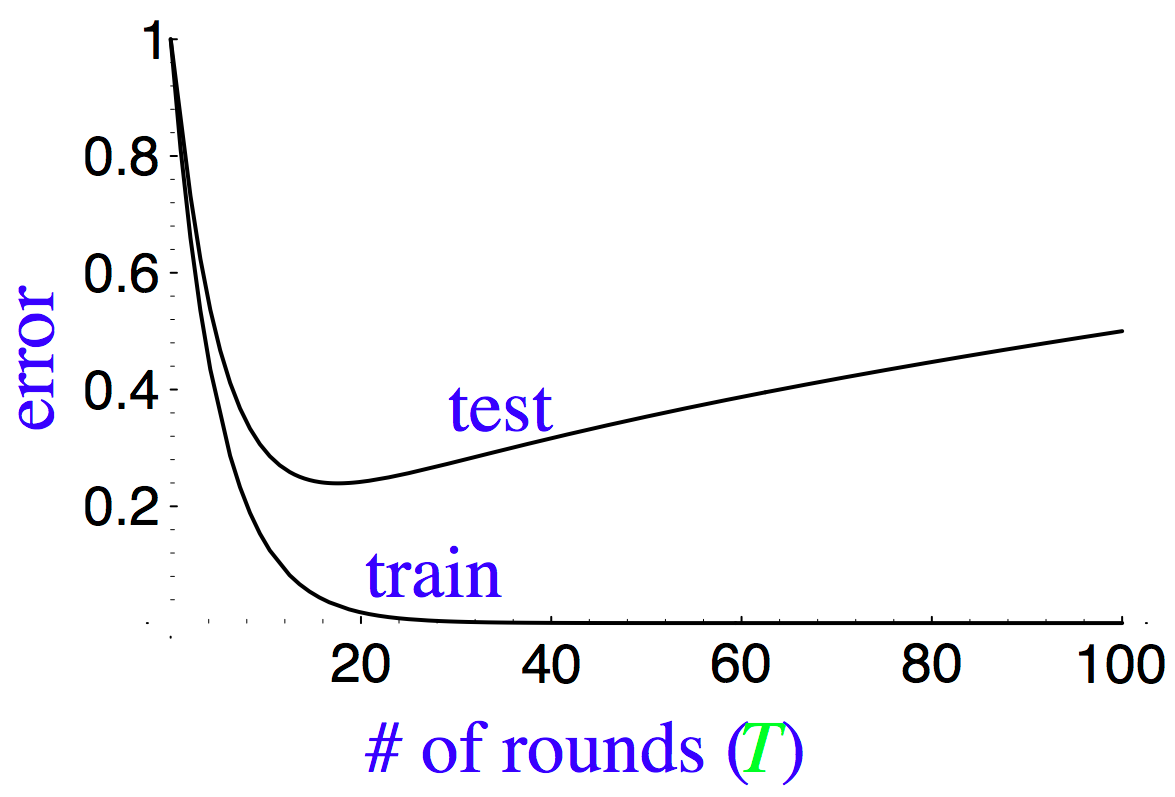
\includegraphics[height=0.55\textheight]{figures/typicalTrainTestCurve}
\par\end{center}

\let\thefootnote\relax\footnotetext{\tiny{From Rob Schapire's NIPS 2007 Boosting tutorial.}}
\end{frame}
%
\begin{frame}{Learning Curves for AdaBoost}
\begin{itemize}
\item AdaBoost is usually quite resistant to overfitting
\item The test error continues to decrease even after the training error drops to zero!
\end{itemize}
\begin{center}
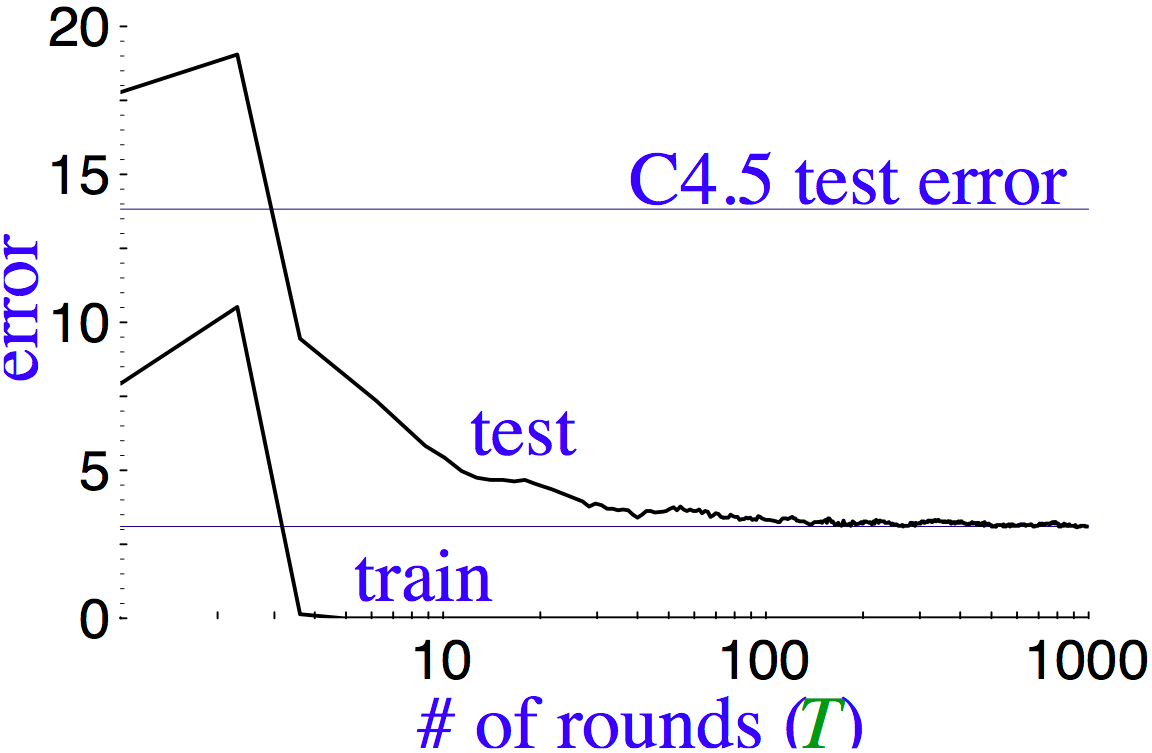
\includegraphics[height=0.55\textheight]{figures/actualTrainTestCurves}
\par\end{center}

\let\thefootnote\relax\footnotetext{\tiny{From Rob Schapire's NIPS 2007 Boosting tutorial.}}
\end{frame}


%%%%%%%%%%%%%%%%%%%%%%%%%%%%%%%%%%%%%%%%%%%%
%%%%%%%%%%%%%%%%%%%%%%%%%%%%%%%%%%%%%%%%%%%%
\begin{frame}{AdaBoost for Face Detection}
\begin{itemize}
\item  Famous application of boosting: detecting faces in images (Viola \& Jones, 2001)
\item A few twists on standard algorithm
\begin{itemize}
    \onslide<2->\item Pre-define weak classifiers, so optimization=selection
    % \onslide<3->\item Change loss function for weak learners: false positives less costly than misses
    \onslide<3->\item Smart way to do inference in real-time (in 2001 hardware)
\end{itemize}
\begin{center}
    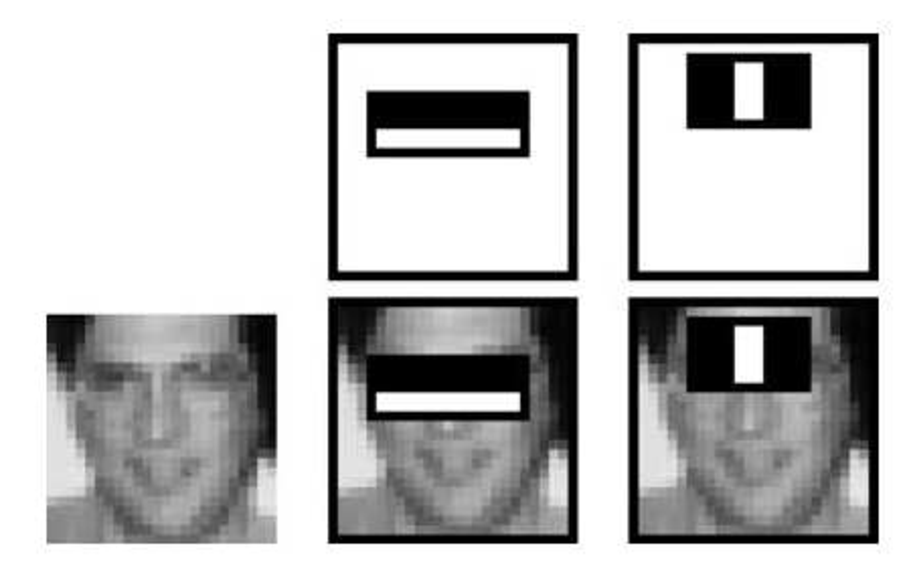
\includegraphics[width=0.4\linewidth]{figures/violajones.pdf} 
\end{center}
\end{itemize}
\end{frame}

\begin{frame}{Harr wavelet basis functions}
\begin{itemize}
    \item A simple way to generate rectangular weights.
    \item Over 180,000 filters on a small image (subwindow) of 24x24.
\end{itemize}
\begin{center}
    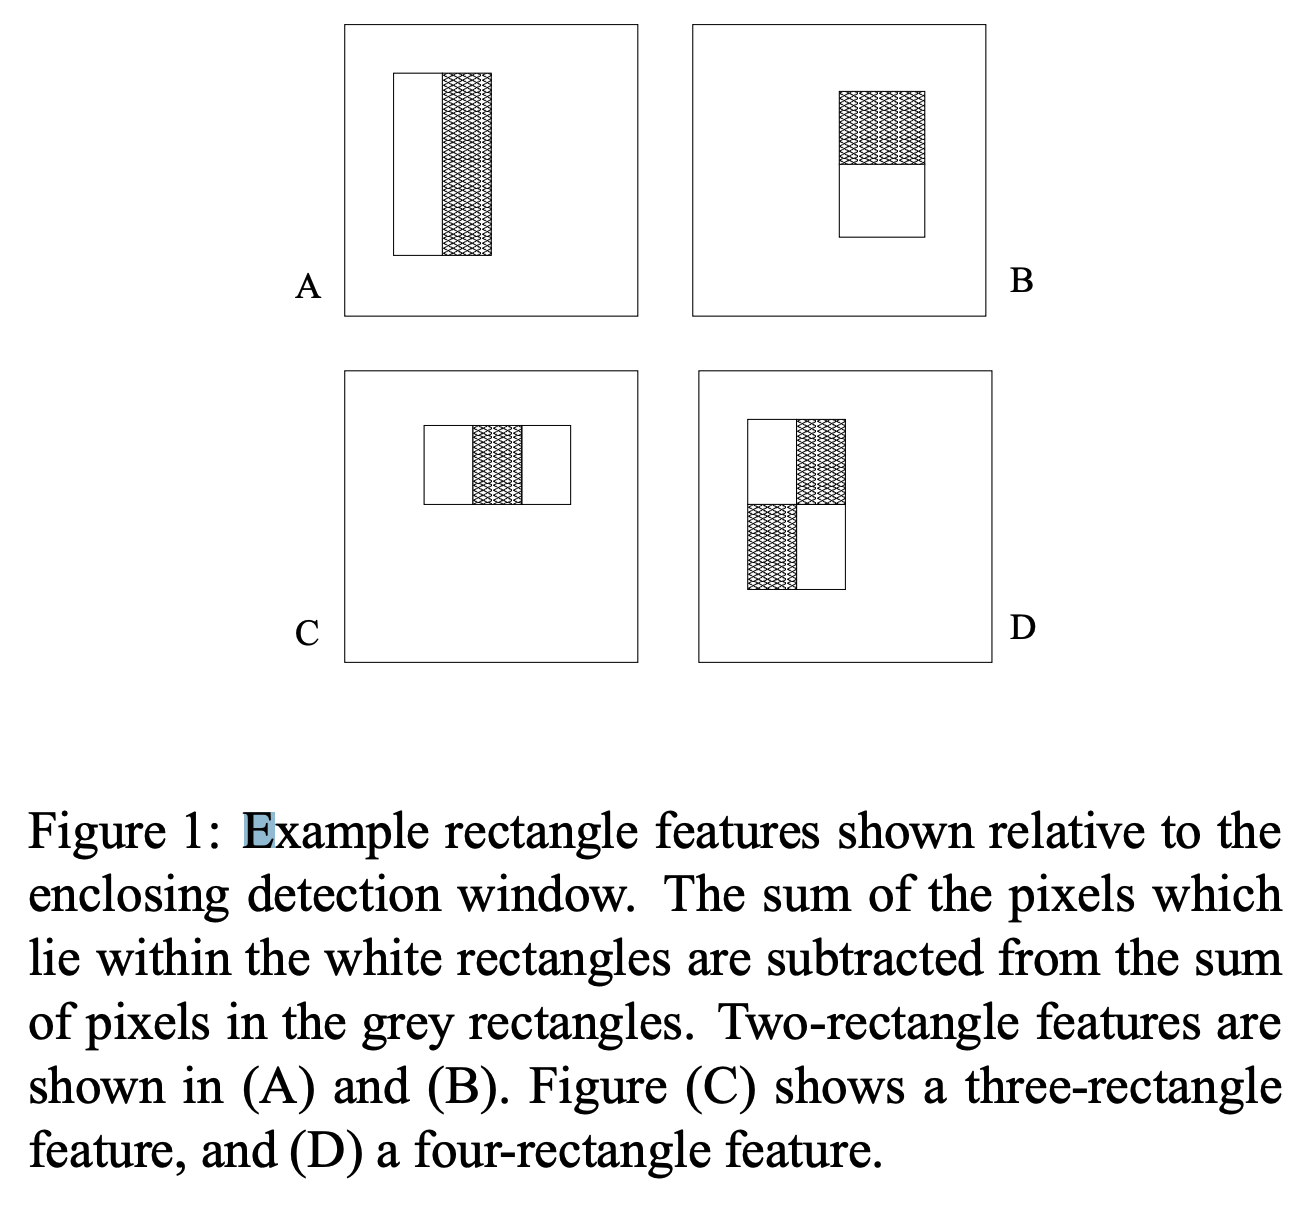
\includegraphics[width=0.4\linewidth]{figures/harr-wavelet.png} 
\end{center}
\end{frame}

\begin{frame}{Integral image}
\begin{itemize}
    \item How to efficiently compute [image * weights] (hint: the sum of an area of the image).
    \item Compute an ``integral image''
    \item Store a 2-D array: S[i, j] = Sum of the image from (0,0) to (i,j).
    \item D = ABCD - AB - AC + A
\end{itemize}
\begin{center}
    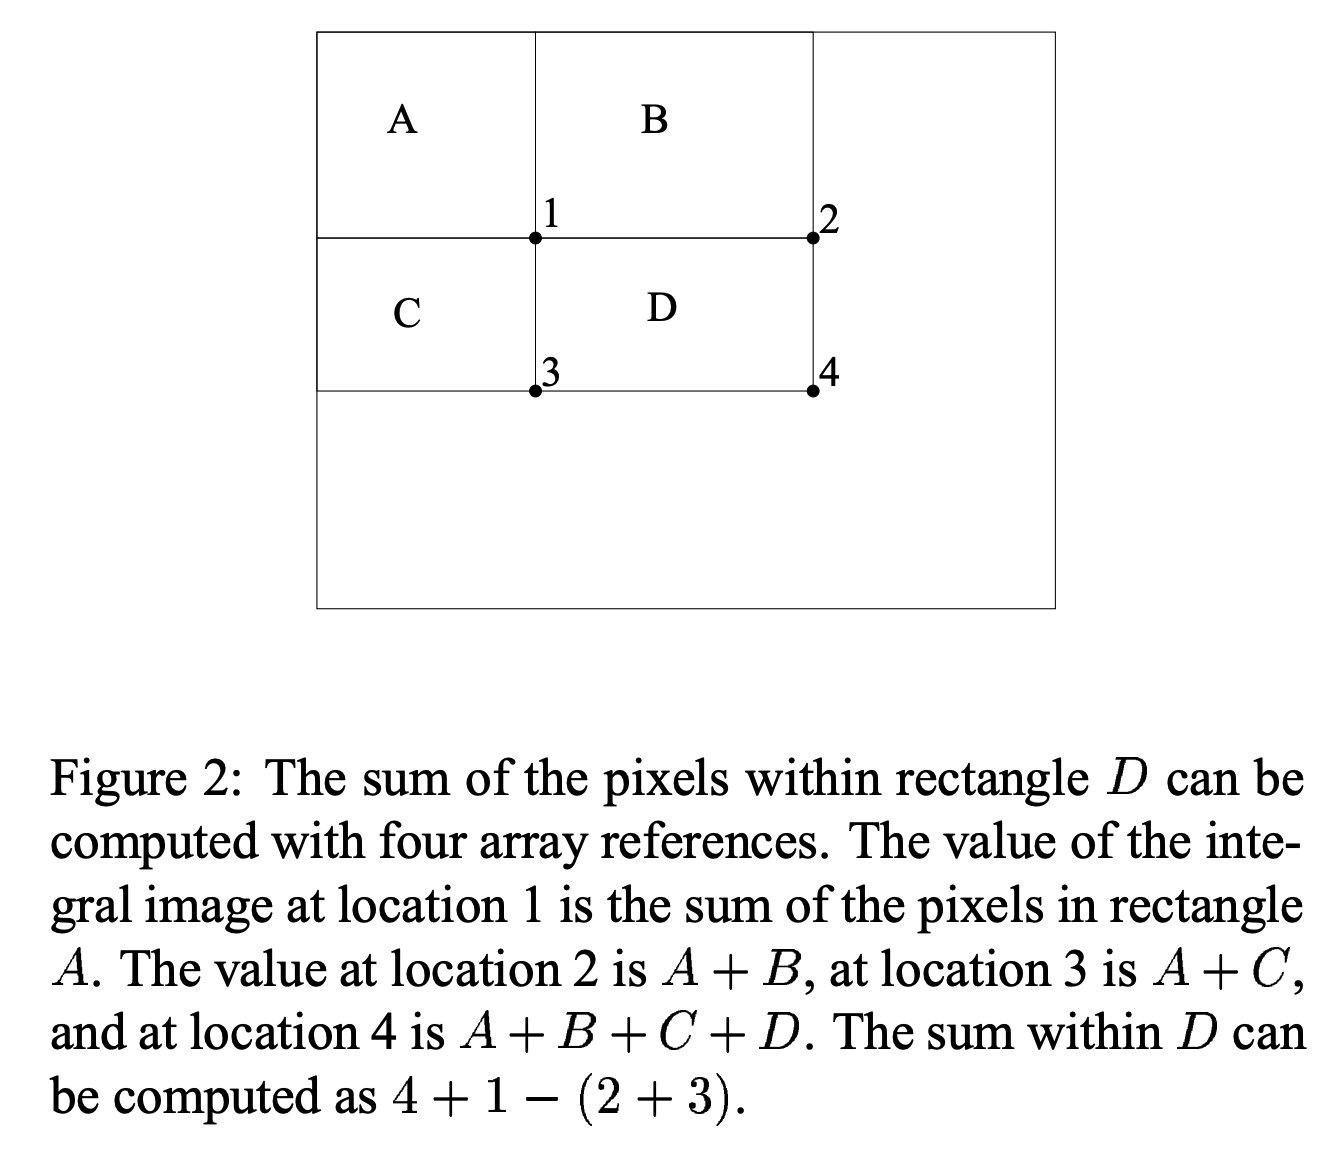
\includegraphics[width=0.4\linewidth, trim={0 9cm 0 0},clip]{figures/integral-image.png} 
\end{center}
\end{frame}


\begin{frame}{Learning Procedure (AdaBoost)}
\begin{itemize}
    \item Review AdaBoost again here, with a slightly different but equivalent setup.
    \item Given example images $(x_1, y_1), \dots, (x_n, y_n)$ where $y_i=0,1$ for negative and positive.
    \pause
    \item Initialize example weights $w_{1,i} = \frac{1}{2m}, \frac{1}{2l}$ for $y_i=0,1$ respectively, where $m$ and $l$ are the number of negatives and positives.
    \pause
    \item For $t = 1, \dots, T$:
    \begin{enumerate}
        \item Normalize the example weights, $w_{t,i} \gets \frac{w_{t,i}}{\sum_{i'=1}^n w_{t,i'}}$
    \pause
        \item For each feature $j$, train a classifier $h_j$. Evaluate weighted error $\epsilon_j = \sum_i w_i |h_j(x_i) - y_i|$.
    \pause
        \item Choose the classifier $h_t$, with the lowest error $\epsilon_t$.
    \pause
        \item Update the example weights:
        $w_{t+1} = w_{t,i} \beta_t^{1-e_i}$, $\beta_t = \frac{\epsilon_t}{1-\epsilon_t}, e_i=0\text{ if correct else } 1$,
    \pause
        \item Final classifier
        $h(x) = \begin{cases}
        1\text{ if } \sum_t \alpha_t h_t(x) > \frac{1}{2} \sum_t \alpha_t \\
        0\text{ otherwise},
        \end{cases}
        \alpha_t = -\log \beta_t
        $
    \end{enumerate}
\end{itemize}
\end{frame}

\begin{frame}{Cascaded Processing for Faster Speed}
\begin{itemize}
    \item Object detection: A large number of subwindows to process.
    \item Do we need to run all the weak classifiers at test time?
    \pause
    \item Threshold can be adjusted so that there is almost no false negative.
    \item False positive is ok. We can reject the windows later.
    \pause
    \item Stop processing if one weak classifier says no.
\end{itemize}
\begin{center}
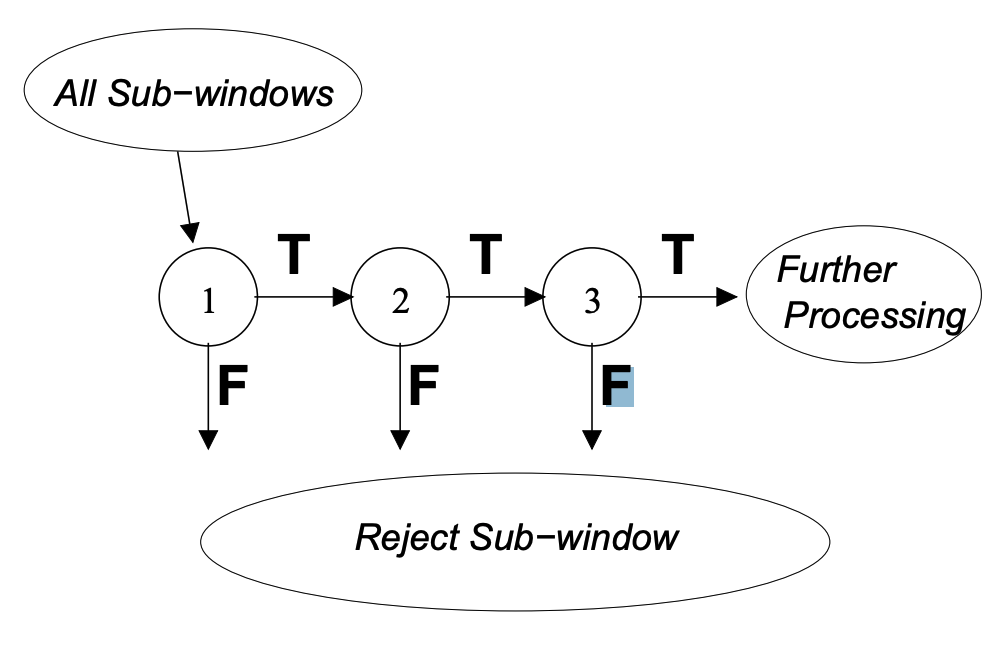
\includegraphics[width=0.35\textwidth]{figures/cascade.png}
\end{center}
\end{frame}
%%%%%%%%%%%%%%%%%%%%%%%%%%%%%%%%%%%%%%%%%%%%
%%%%%%%%%%%%%%%%%%%%%%%%%%%%%%%%%%%%%%%%%%%%
\begin{frame}{AdaBoost Face Detection Results}
\vspace{-0.2cm}
\begin{center}

\includegraphics[width=0.5\linewidth]{figures/adaboost_facedetection} 
\end{center}
\end{frame}

\begin{frame}
{Interim Summary}
    \begin{itemize}[<+->]
\item Boosting is used to reduce bias from shallow decision trees
\item Each classifier is trained to reduce errors of its previous ensemble.
\item AdaBoost is a very powerful off-the-self classifier.
\item A real-time face detection algorithm made by AdaBoost.
% \item Next week
\begin{itemize}
\item What is the objective function of AdaBoost?
\item Generalizations to other loss functions
\item Gradient Boosting
\end{itemize}
\end{itemize}
\end{frame}

\begin{frame}
{Gradient Boosting}
\begin{itemize}
\item Another way to get non-linear models in a linear form---adaptive basis function models.
\item A general algorithm for greedy function approximation---gradient boosting machine.
    \begin{itemize}
        \item Adaboost is a special case.
    \end{itemize}
\end{itemize}
\note[item]{We've learned kernel methods which gives you a non-linear classifier in a linear form. Today we are going to learn another method called ``adaptive basis function models''.
}
\note[item]{And we are going to learn a general algorithm for learning these basis functions, which give rise to a family of boosting algorithms, including Adaboost we saw last time.}
\end{frame}

\section{Motivation}
\begin{frame}
{Recap: Adaboost}
\begin{center}
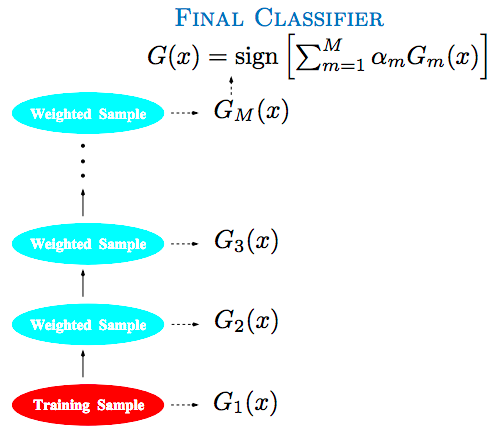
\includegraphics[height=0.7\textheight]{figures/adaboostSchematic}
\par\end{center}
\let\thefootnote\relax\footnotetext{\tiny{From ESL Figure 10.1}}
\note[item]{Recall the Adaboost algorithm we talked about last time. We want to learn a sequence of base classifiers; each of them minimizes weighted zero-one error, where the weights are higher on previously misclassified examples. It's like when you study for an exam, you go over all practice questions; then you look at the answers. The next time you spend more time on questions you go wrong. In the end you would grasp everything.}
\note[item]{Our final classifier is a weighted combination the base classifiers. The weights on good classifiers are higher, where ``good'' is measured by weighted zero-one error.}
\note[item]{Last time we went over a greedy algorithm for obtaining the base classifiers and the weights. Let's review the Adaboost algorithm.}
\end{frame}

\begin{frame}{AdaBoost: Algorithm}

Given training set $\cd=\left\{ \left(x_{1},y_{1}\right),\ldots,\left(x_{n},y_{n}\right)\right\} $.
\begin{enumerate}
\item Initialize observation weights $w_{i}=1$, $i=1,2,\ldots,n$.

\item For $m=1$ to $M$:
\begin{enumerate}
\item Base learner fits weighted training data and returns $G_{m}(x)$

\item Compute \emph{weighted empirical 0-1 risk}:
\[
\mbox{err}_{m}=\frac{1}{W}\sum_{i=1}^{n}w_{i}\ind{y_{i}\neq G_{m}(x_{i})}\quad\text{where }W=\sum_{i=1}^{n}w_{i}.
\]

\item Compute  \emph{classifier weight}: $\alpha_{m}=\ln\left(\frac{1-\text{err}_{m}}{\text{err}_{m}}\right)$.

\item Update \emph{example weight}: $w_{i}\gets w_{i}\cdot\exp\left[\alpha_{m}\ind{y_{i}\neq G_{m}(x_{i})}\right]$
\end{enumerate}
\item Return \emph{voted classifier}: $G(x)=\sign\left[\sum_{m=1}^{M}\alpha_{m}G_{m}(x)\right]$.
\onslide<+->{\hspace{2em}{\color{red}Why not learn $G(x)$ directly?}}
\end{enumerate}
%\note[item]{But why does this algorithm work? Does it actually gives us a good classifier in our hypothesis space? Let's work backwards. Since $G(x)$ is the final model we want, why don't we learn it directly? This is actually a special case of additive basis function models.}
\note[item]{Now that we have a hypothesis space, and a loss function depending on whether we are doing classification or regression, why don't we follow our familiar recipe to write down the ERM objective, and run gradient descent to learn the parameters.}
\end{frame}

\begin{frame}{Nonlinear Regression}
\begin{itemize}
\item How do we fit the following data?
\begin{figure}
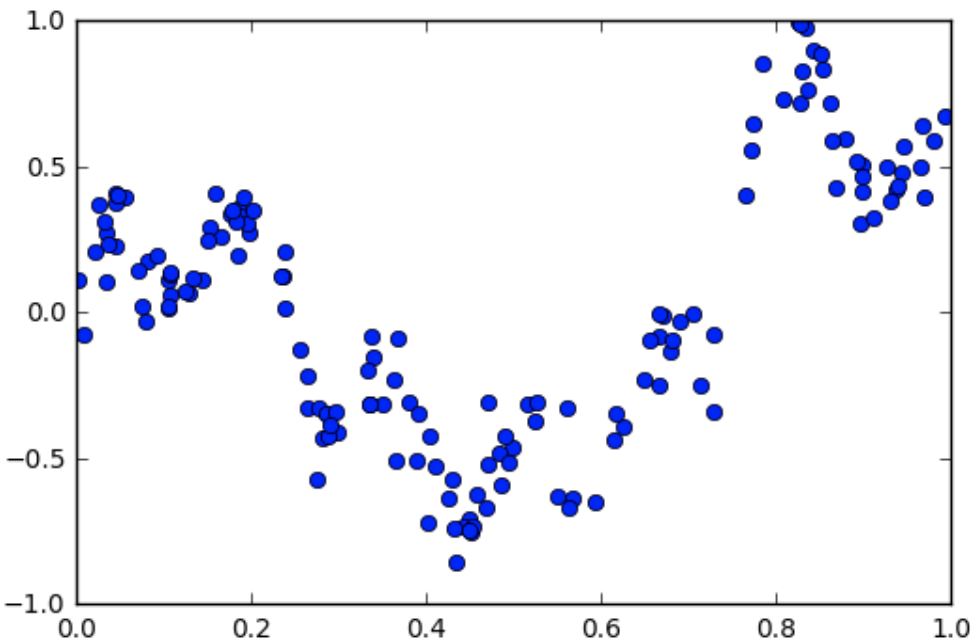
\includegraphics[height=0.6\textheight]{figures/nonlinear-regression-data}
\end{figure}
\end{itemize}
\note[item]{To motivate adaptive basis models, let's consider this nonlinear regression problem. Given the following data, what model would you use?}
\note[item]{We can create non-linear features.}
\end{frame}
%
\begin{frame}{Linear Model with Basis Functions}
\begin{itemize}[<+->]
\item Fit a linear combination of transformations of the input:
\[
f(x)=\sum_{m=1}^{M}v_{m}h_{m}(x),
\]
where $h_m$'s are called \textbf{basis functions} (or feature functions in ML):
\[
h_{1},\ldots,h_{M}:\cx\to\reals
\]
\item Example: polynomial regression where $h_m(x) = x^m$.
\item Can we use this model for classification?
\note[item]{$f(x)$ can be transformed to a probability (\eg similar to GLM), or used as a score function (\eg margin-based classification and ranking).}
\item Can fit this using standard methods for linear models (e.g. least
squares, lasso, ridge, etc.)
\begin{itemize}
\item \emph{Note that $h_m$'s are fixed and known}, \ie chosen ahead of time.
\end{itemize}
\end{itemize}
\note[item]{The key idea here is to use a family of functions or transformations that can be applied to $x$, which are called basis functions.}
\note[item]{The basis functions can be non-linear in $x$. Can you think of some examples? Polynomials, piecewise constant functions.}
\note[item]{We can use it for classification by another function to transform the results to a probability or a class, \eg sgn as in Adaboost.}
\note[item]{All inference methods we've learned for linear models can be applied here. Why? It's important to note that $h_m$ are fixed, thus they can be simply considered as another feature.}
\end{frame}
%
\begin{frame}{Adaptive Basis Function Model}
\begin{itemize}[<+->]
\item What if we want to learn the basis functions? (hence \emph{adaptive})

\item {Base hypothesis space} $\ch$ consisting of functions $h:\cx\to\reals$.

\item<.-> An \textbf{adaptive basis function expansion }over $\ch$ is
an ensemble model:
\begin{align}
f(x)=\sum_{m=1}^{M}v_{m}h_{m}(x),
\end{align}
where $v_{m}\in\reals$ and $h_{m}\in\ch$.

\item Combined hypothesis space:
\[
\cf_{M}=\left\{ \sum_{m=1}^{M}v_{m}h_{m}(x)\mid v_{m}\in\reals,\:h_{m}\in\ch,\:m=1,\ldots,M\right\} 
\]
\item<.-> What are the learnable?
\end{itemize}
\note[item]{But in Adaboost we don't know the base classifier beforehand. How to learn them?}
\note[item]{Let's formalize the problem a bit. The basis functions belong to the base hypothesis space, and our predictor is a linear combination of the basis functions, just as every vector in a vector space can be represented by a linear combination of the basis vectors.}
\note[item]{Both the weights $v_m$ and  the basis functions $h_m$ are learned, as in Adaboost.}
\end{frame}
%
%\begin{frame}{Adaptive Basis Function Model}
%\begin{itemize}
%\item \textbf{Base hypothesis space}: $\ch$ of \textbf{real-valued functions} 
%\item \textbf{Combined hypothesis space:} $\cf_{M}$:
%\[
%\cf_{M}=\left\{ \sum_{m=1}^{M}v_{m}h_{m}(x)\mid v_{m}\in\reals,\:h_{m}\in\ch,\:m=1,\ldots,M\right\} 
%\]
%
%\pause{}
%\item Suppose we're given some data $\cd=\left((x_{1},y_{1}),\ldots,(x_{n},y_{n})\right)$.
%
%\pause{}
%\item Learning is choosing $v_{1},\ldots,v_{M}\in\reals$ and $h_{1},\ldots,h_{M}\in\ch$
%to fit $\cd$.
%\end{itemize}
%\end{frame}

%\begin{frame}{Not Limited to Regression}
%\begin{itemize}
%\item Linear combination of basis functions:
%\[
%f(x)=\sum_{m=1}^{M}v_{m}g_{m}(x)
%\]
%\item $f(x)$ is a number \textemdash{} for regression, it's exactly what
%we're looking for.
%
%\pause{}
%\item Otherwise, $f(x)$ is often called a \textbf{score} function.
%\item It can be 
%\begin{itemize}
%\item thresholded to get a classification
%\item transformed to get a probability
%\item transformed to get a parameter of a probability distribution (e.g.
%Poisson regression)
%\item used for ranking search results
%\end{itemize}
%\end{itemize}
%\end{frame}
%

%
\begin{frame}{Empirical Risk Minimization}
\begin{itemize}[<+->]
\item What's our learning objective? 
\[
\hat{f}=\argmin_{f\in\cf_{M}}\frac{1}{n}\sum_{i=1}^{n}\ell\left(y_{i},f(x_{i})\right),
\]
for some {loss function} $\ell$. 

\item Write ERM objective function as
\[
J(v_{1},\ldots,v_{M},h_{1},\ldots,h_{M})=\frac{1}{n}\sum_{i=1}^{n}\ell\left(y_{i},\sum_{m=1}^{M}v_{m}h_{m}(x)\right).
\]

\item How to optimize $J$? i.e. how to learn?
\end{itemize}
\note[item]{So the main question left is how to optimize $J$. Adaboost uses a greedy algorithm. But can we directly optimize all parameters?}
\end{frame}
%
\begin{frame}{Gradient-Based Methods}
\begin{itemize}[<+->]
\item \texttt{Suppose} our base hypothesis space is parameterized by $\Theta=\reals^{b}$:
\[
J(v_{1},\ldots,v_{M},{\color{blue}\theta_{1},\ldots,\theta_{M}})=\frac{1}{n}\sum_{i=1}^{n}\ell\left(y_{i},\sum_{m=1}^{M}v_{m}h(x;{\color{blue}\theta_{m}})\right).
\]

\item Can we optimize it with SGD?
\begin{itemize}
\item Can we differentiate $J$ w.r.t. $v_{m}$'s and $\theta_{m}$'s?
\end{itemize}

\item For {some} hypothesis spaces and typical loss functions, yes!
\begin{itemize}[<.->]
\item Neural networks fall into this category! ($h_{1},\ldots,h_{M}$ are
neurons of last hidden layer.)
\end{itemize}
\end{itemize}
\note[item]{Note that $h$ doesn't have to be a parametric model; it can be non-parametric, \eg decision trees.}
\note[item]{Running SGD requires the objective to be differentiable w.r.t. the parameters, \eg neural networks.}
\end{frame}
%
\begin{frame}{What if Gradient Based Methods Don't Apply?}
\begin{simpleblock}
{{What if base hypothesis space $\ch$ consists of decision trees?}}
\begin{itemize}[<2->]
\item Can we even parameterize trees with $\Theta=\reals^{b}$?
\item Even if we could, predictions would not change continuously w.r.t. $\theta\in\Theta$, so certainly not differentiable.
\end{itemize}
\end{simpleblock}
\note[item]{First of all, we cannot really parametrize decision trees as the number of parameters depends on the tree structure. But even if we fix the tree structure, in which case the parameters are the splitting feature values, we still cannot run SGD as the function is piecewise-constant.}

\begin{simpleblock}
{\onslide<3->{What about a greedy algorithm similar to Adaboost?}}
\begin{itemize}[<4->]
\item Applies to non-parametric or non-differentiable basis functions.
\item But is it optimizing our objective using some loss function?
\end{itemize}
\end{simpleblock}
\note[item]{Adaboost gives us a model in the form of an adaptive basis function model. But what the objective function it is optimizing?}
\end{frame}

\begin{frame}
\begin{simpleblock}
{Today we'll discuss \textbf{gradient boosting}.}
\begin{itemize}
\item Gradient descent in the \emph{function space}.
\item It applies whenever 
\begin{itemize}
\item our loss function is {[}sub{]}differentiable w.r.t. training predictions
$f(x_{i})$, and
\item we can do regression with the base hypothesis space $\ch$.
\end{itemize}
\end{itemize}
\end{simpleblock}

\note[item]{Using gradient boosting, we can directly optimize the basis functions in the function space.}
\note[item]{We will show that Adaboost is just a special case of gradient boosting using the exponential loss.}
\note[item]{This algorithm is very general, it only requires...}
\end{frame}
%

% \begin{frame}
% {History}
% \begin{table}
% \begin{tabular}{rp{8cm}}
% Kearns, Valiant (1989): & Can weak learners (\eg $51\%$ accuracy) be transformed to strong learners (\eg $99.9\%$ accuracy)?
% % \pause 
% \\
% Schapire (1990) \& Freund (1995): & Yes, weak learners can be iteratively improved to a strong learner.
% % \pause 
% \\
% Freund, Schapire (1996): & And here is a practical algorithm---Adaboost.
% % \pause 
% \\
% Breiman (1996 \& 1998): & Yes, it works! Boosting is the best off-the-shelf classifier in the world.
% % \pause 
% \\
% \multicolumn{2}{c}{(Attempts to explain why Adaboost works and improvements)}
% % \pause
% \\
% Friedman, Hastie, Tibshirani (2000): & Actually, boosting fits an additive model.\pause \\
% Friedman (2001): & Furthermore, it can be considered as gradient descent in the function space.
% \end{tabular}
% \end{table}
%     \note[item]{Adaboost is a great example where a pure theoretical investigation leads to huge practical success.}
% \note[item]{The idea of boosting started from a theoretical question: can we transform weak learners that are merely better than chance to arbitrarily strong learners?}
% \note[item]{Schapir and Freund first gave an affirmative answer. However their boosting algorithm at that time was mainly constructed for theoretical proofs. In 1996, Adaboost was born.}
% \note[item]{There is a lot of excitement in the ML community around it. In particular, Leo Breiman, who contributed many ideas we learned last week including CART, bagging, and random forest, said that...}
% \note[item]{Then there are many attempts to explain why it works, variations and improvements. Finally, in 2000, FHT (the authors of one of our reference books, ESL) gave a statistical view of boosting. It in fact fits an additive model.}
% \note[item]{Friedman further elaborates the idea using gradient descent in the function space, which we will learn about today.}
% \end{frame}

%\begin{frame}{Overview}
%\begin{itemize}
%\item Forward stagewise additive modeling (FSAM)
%\begin{itemize}
%\item example: $L^{2}$ Boosting 
%\item example: exponential loss gives AdaBoost
%\item Not clear how to do it with many other losses, including logistic
%loss
%\end{itemize}
%\item Gradient Boosting
%\begin{itemize}
%\item example: logistic loss gives BinomialBoost
%\end{itemize}
%\item Variations on Gradient Boosting
%\begin{itemize}
%\item step size selection
%\item stochastic row/column selection
%\item Newton step direction
%\item XGBoost
%\end{itemize}
%\end{itemize}
%\end{frame}

\section{Forward Stagewise Additive Modeling }
\begin{frame}{Forward Stagewise Additive Modeling (FSAM)}
\begin{description}
\item[Goal] fit model $f(x) = \sum_{m=1}^M v_mh_m(x)$ given some loss function.
\item[Approach]
{Greedily} fit one function at a time without adjusting previous functions, hence ``forward stagewise''.
\end{description}

\begin{itemize}[<+->]
\item After $m-1$ stages, we have
\[
f_{m-1}=\sum_{i=1}^{m-1}v_{i}h_{i}.
\]
 
\item In $m$'th round, we want to find 
$h_{m}\in\ch$ (i.e. a basis function) and
$v_{m}>0$ 
such that 
\[
f_{m}=\underbrace{f_{m-1}}_{\text{fixed}}+v_{m}h_{m}
\]
improves objective function value by as much as possible.
\end{itemize}
\note[item]{At the $m$'th stage, we would have trained $m-1$ classifiers, so the current classifier is a combination of the previous $m-1$ classifiers.}
\note[item]{And we will fit the next basis function $h_m$ and $v_m$ to improve the objective function value as much as possible. Here we consider $f_{m-1}$ fixed and known.
Note that in each round, we are only doing local improvement w.r.t. the $m$'th basis function.}
\end{frame}
%
\begin{frame}{Forward Stagewise Additive Modeling for ERM}
Let's plug in our objective function.
\begin{enumerate}
\item Initialize $f_{0}(x)=0$.
\item For $m=1$ to $M$:

\pause{}
\begin{enumerate}
\item Compute:
\[
\left(v_{m},h_{m}\right)=\argmin_{v\in\reals,h\in\ch}\frac{1}{n}\sum_{i=1}^{n}\ell\left(y_{i},f_{m-1}(x_{i})\underbrace{+v h(x_{i})}_{\text{new piece}}\right).
\]


\pause{}
\item Set $f_{m}=f_{m-1}+v_{m}h_m$.

\pause{}
\end{enumerate}
\item Return: $f_{M}$.
\end{enumerate}
\note[item]{We fit $M$ basis functions sequentially. In each round, we find the next basis function $h_m$ and its weight $v_m$ that minimizes the empirical risk.
And we add that to our current model $f$.}
\note[item]{In the end, we return a weighted sum of the $M$ basis functions.}
\note[item]{Next, we will show that Adaboost is FSAM with exponential loss.}
\end{frame}
%

\subsection{Example: AdaBoost}
% \begin{frame}{Recap: margin-based classifier}
% \begin{simpleblock}
% {Binary classification}
% \begin{itemize}
% \item Outcome space $\cy=\left\{ -1,1\right\} $
% \item Action space $\ca=\reals$ (model outoput)
% \item Score function $f:\cx\to\ca$.
% \item Margin for example $(x,y)$ is $m=yf(x)$. 
% \begin{itemize}
% \item $m>0\iff$ classification correct
% \item Larger $m$ is better.
% \end{itemize}
% \item \think{Concept check}: What are margin-based loss functions we've seen?
% \end{itemize}
% \end{simpleblock}
% \note[item]{Exponential loss is a margin-based loss function. Before talking about the exponential loss, let's first do a quick recap of margin-based classifier.}
% \note[item]{Other margin-based loss: hinge loss, logistic loss in HW5.}
% \end{frame}
%
%
\begin{frame}{Exponential Loss}
\begin{itemize}
\item Introduce the \textbf{exponential loss}: $\ell(y,f(x))=\exp\left(-\underbrace{yf(x)}_{\text{margin}}\right).$
\end{itemize}
\begin{center}
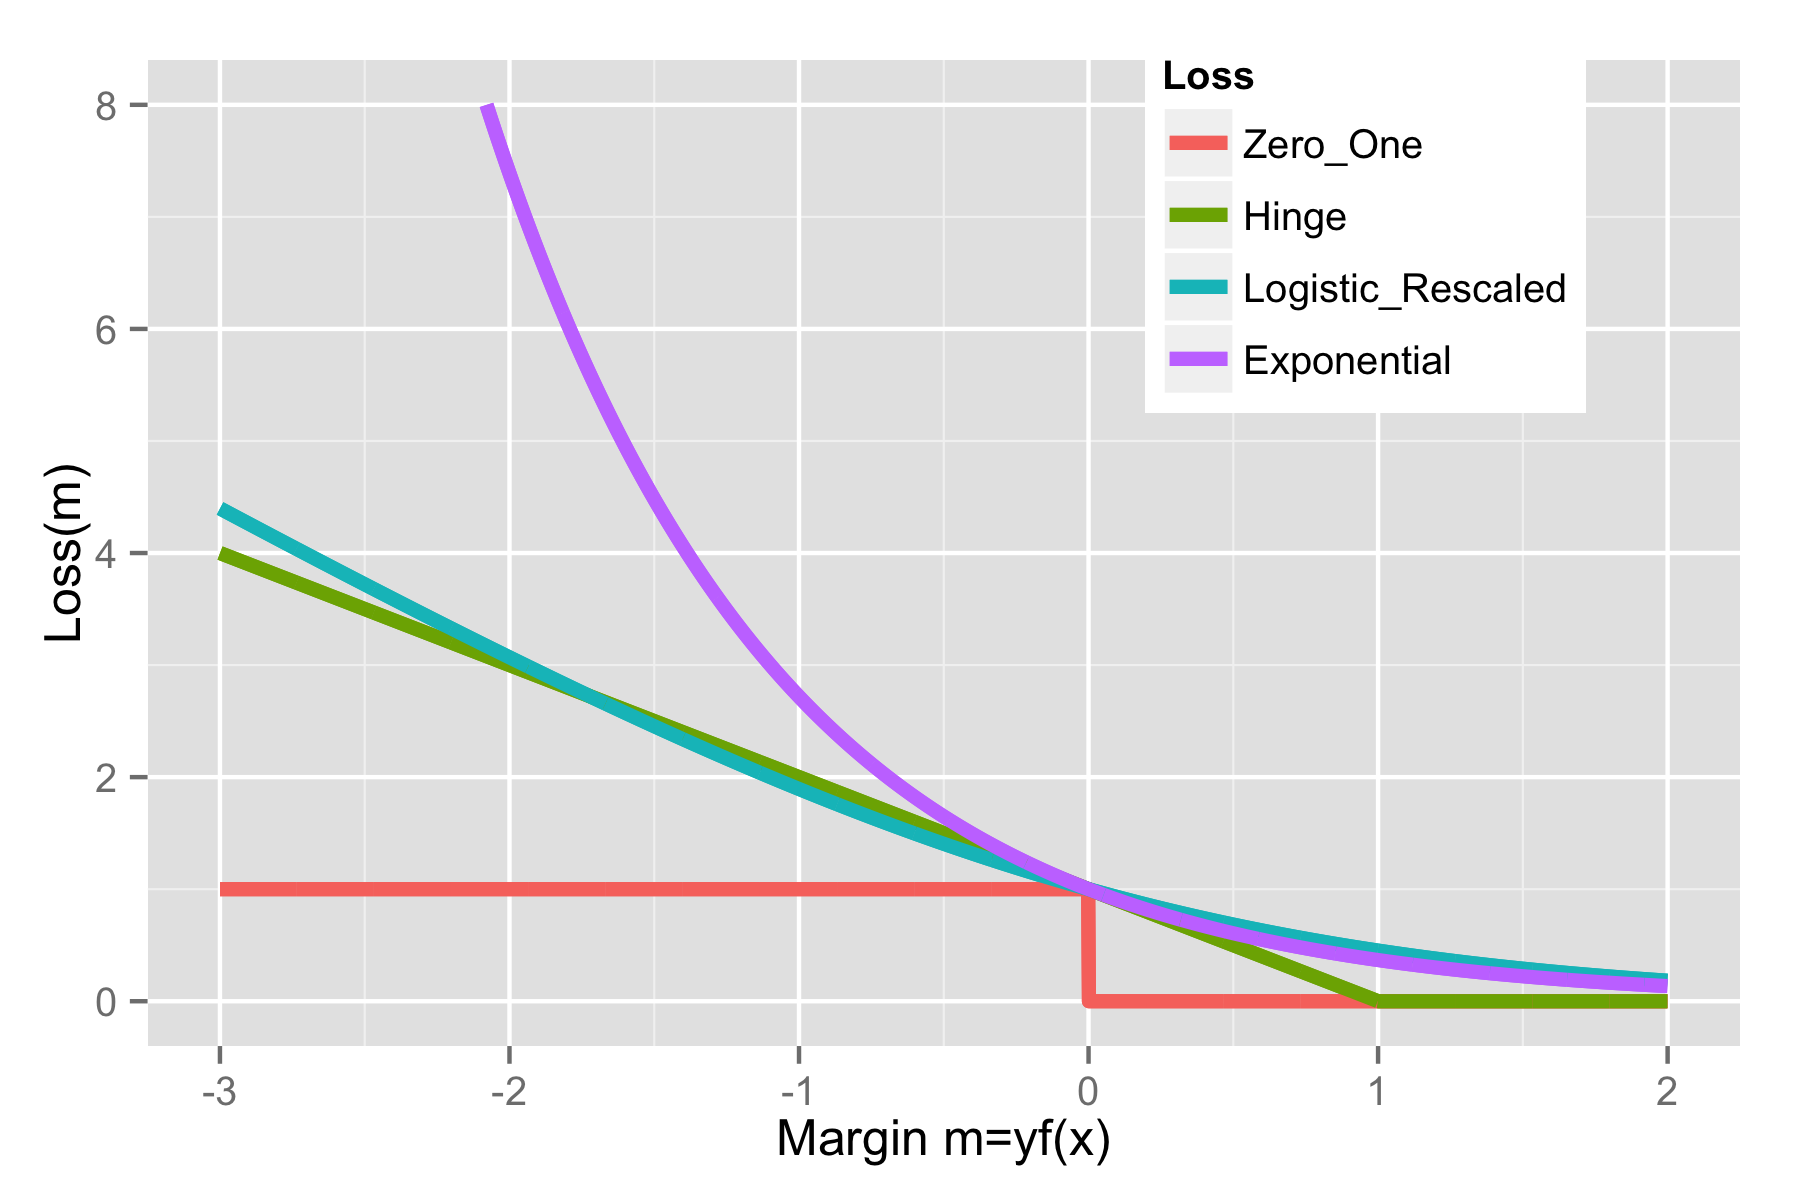
\includegraphics[height=0.65\textheight]{{figures/loss.Zero_One.Hinge.Logistic_Rescaled.Exponential}.png}
\par\end{center}
\note[item]{The exponential loss is just the exponential of negative margin. It is also a convex upperbound of the zero-one loss.}
\end{frame}
%
\begin{frame}{Forward Stagewise Additive Modeling with exponential loss}
Recall that we want to do FSAM with exponential loss.
\begin{enumerate}
\item Initialize $f_{0}(x)=0$.
\item For $m=1$ to $M$:
\begin{enumerate}
\item Compute:
\[
\left(v_{m},h_{m}\right)=\argmin_{v\in\reals,h\in\ch}\frac{1}{n}\sum_{i=1}^{n}{\color{blue}\ell_{\text{exp}}}\left(y_{i},f_{m-1}(x_{i})\underbrace{+v h(x_{i})}_{\text{new piece}}\right).
\]
\item Set $f_{m}=f_{m-1}+v_{m}h_m$.
\end{enumerate}
\item Return: $f_{M}$.
\end{enumerate}
\note[item]{Now let's plug in our loss function in FSAM.}
\end{frame}

\begin{frame}{FSAM with Exponential Loss: objective function}
\begin{itemize}
\item Base hypothesis: $\sH = \pc{h\colon \sX \rightarrow \pc{-1, 1}}$.
\item Objective function in the $m$'th round:
\pause
\begin{align}
J(v, h) &= \sum_{i=1}^n \exp\pb{
-y_i \p{ f_{m-1}(x_i) + vh(x_i) }
} \\
&= \sum_{i=1}^n w_i^m \exp\pb{ -y_ivh(x_i) } &&  \commenteq{w_i^m \eqdef \exp\pb{ -y_i f_{m-1}(x_i) } }\\
&= \sum_{i=1}^n w_i^m \pb{ \1\p{y_i=h(x_i)}e^{-v} + \1\p{y_i\neq h(x_i)}e^v } 
&& \commenteq{h(x_i) \in \pc{1, -1}} \\
&=  \sum_{i=1}^n w_i^m \pb{ (e^v-e^{-v})\1\p{y_i\neq h(x_i)} + e^{-v} }
&& \commenteq{\1\p{y_i=h(x_i)} = 1- \1\p{y_i\neq h(x_i)}}
\end{align}


\end{itemize}
\end{frame}
%
\begin{frame}{FSAM with Exponential Loss: basis function}
\begin{itemize}[<+->]
\item Objective function in the $m$'th round:
\begin{align}
J(v, h) &= \sum_{i=1}^n w_i^m \pb{ (e^v-e^{-v})\1\p{y_i\neq h(x_i)} + e^{-v} } .
\end{align}
\item If $v>0$, then
\begin{align}
\onslide<.->{
\argmin_{h\in\sH}J(v,h) &=
\argmin_{h\in\sH} \sum_{i=1}^n w_i^m \1\p{y_i\neq h(x_i)} \\
}
\onslide<+->{
h_m &= \argmin_{h\in\sH} \sum_{i=1}^n w_i^m \1\p{y_i\neq h(x_i)} \\
}
\onslide<+->{
&= \argmin_{h\in\sH} \frac{1}{\sum_{i=1}^n w_i^m} \sum_{i=1}^n w_i^m \1\p{y_i\neq h(x_i)}
&& \commenteq{\text{multiply by a positive constant}}
}
\end{align}
\onslide<+->{
\ie $h_m$ is the minimizer of the weighted zero-one loss.
}
\end{itemize}
\note[item]{Let's first find the optimal $h$, the last term does not depend on $h$ so it can be ignored for now. Do we want the indicator to be one or zero? It depends on the coefficient.}
\end{frame}

\begin{frame}{FSAM with Exponential Loss: classifier weights}
\begin{itemize}[<+->]
\item Define the weighted zero-one error:
\begin{align}
\text{err}_m = \frac{\sum_{i=1}^n w_i^m \1\p{y_i\neq h(x_i)}}{\sum_{i=1}^n w_i^m} .
\end{align}
\item \think{Exercise}: show that the optimal $v$ is:
\begin{align}
v_m = \frac{1}{2}\log\frac{1-\text{err}_m}{\text{err}_m}
\end{align}
\begin{itemize}
\item Same as the classifier weights in Adaboost (differ by a constant).
\item If $\text{err}_m < 0.5$ (better than chance), then $v_m > 0$.
\end{itemize}
\end{itemize}
\note[item]{Now let's fine the optimal weight $v$.}
\note[item]{To simplify notation, let's define $err_m$. Since $v$ is a real number, you can compute the gradient w.r.t. $v$ and set it to zero.}
\note[item]{Remember that we assumed $v>0$. Is it true for optimal $v$?}
\end{frame}

\begin{frame}
{FSAM with Exponential Loss: example weights}
\begin{itemize}
\item Weights in the next round:
\begin{align}
w_i^{m+1} &\eqdef \exp\pb{ -y_i f_m(x_i) } \\
\onslide<2->{
&= w_i^m \exp\pb{ -y_i v_m h_m(x_i) } 
\quad\quad\quad \commenteq{f_m(x_i) = f_{m-1}(x_i) + v_mh_m(x_i)} \\
&= w_i^m \exp\pb{ -v_m\1\p{y_i = h_m(x_i)} + v_m\1\p{y_i \neq h_m(x_i)} } \\
&= w_i^m \exp\pb{ 2v_m\1\p{y_i \neq h_m(x_i)} } \underbrace{\exp^{-v_m}}_{\text{scaler}}
}
\end{align}
\item<3-> The constant scaler will cancel out during normalization.
\item<4-> $2v_m = \alpha_m$ in Adaboost.
\end{itemize}
\note[item]{So far we have shown that FSAM with exponential loss also fits base classifiers using the weighted zero-one loss, and classifier weights is the same as Adaboost. But what about the example weights?}
\note[item]{The example weights are updated in the same way too! If an example is misclassified, we increase its weight same as in Adaboost.}
\note[item]{Now we have derived Adaboost using FSAM with exponential loss.}
\end{frame}

\begin{frame}{Why Exponential Loss}
\begin{itemize}[<+->]
\item $\ell_{\text{exp}}(y, f(x)) = \exp(-yf(x))$.
\item \think{Exercise}: show that the optimal estimate is
\begin{align}
f^*(x) = \frac{1}{2}\log\frac{p(y=1\mid x)}{p(y=0\mid x)} .
\end{align}
\item How is it different from other losses?
\begin{center}
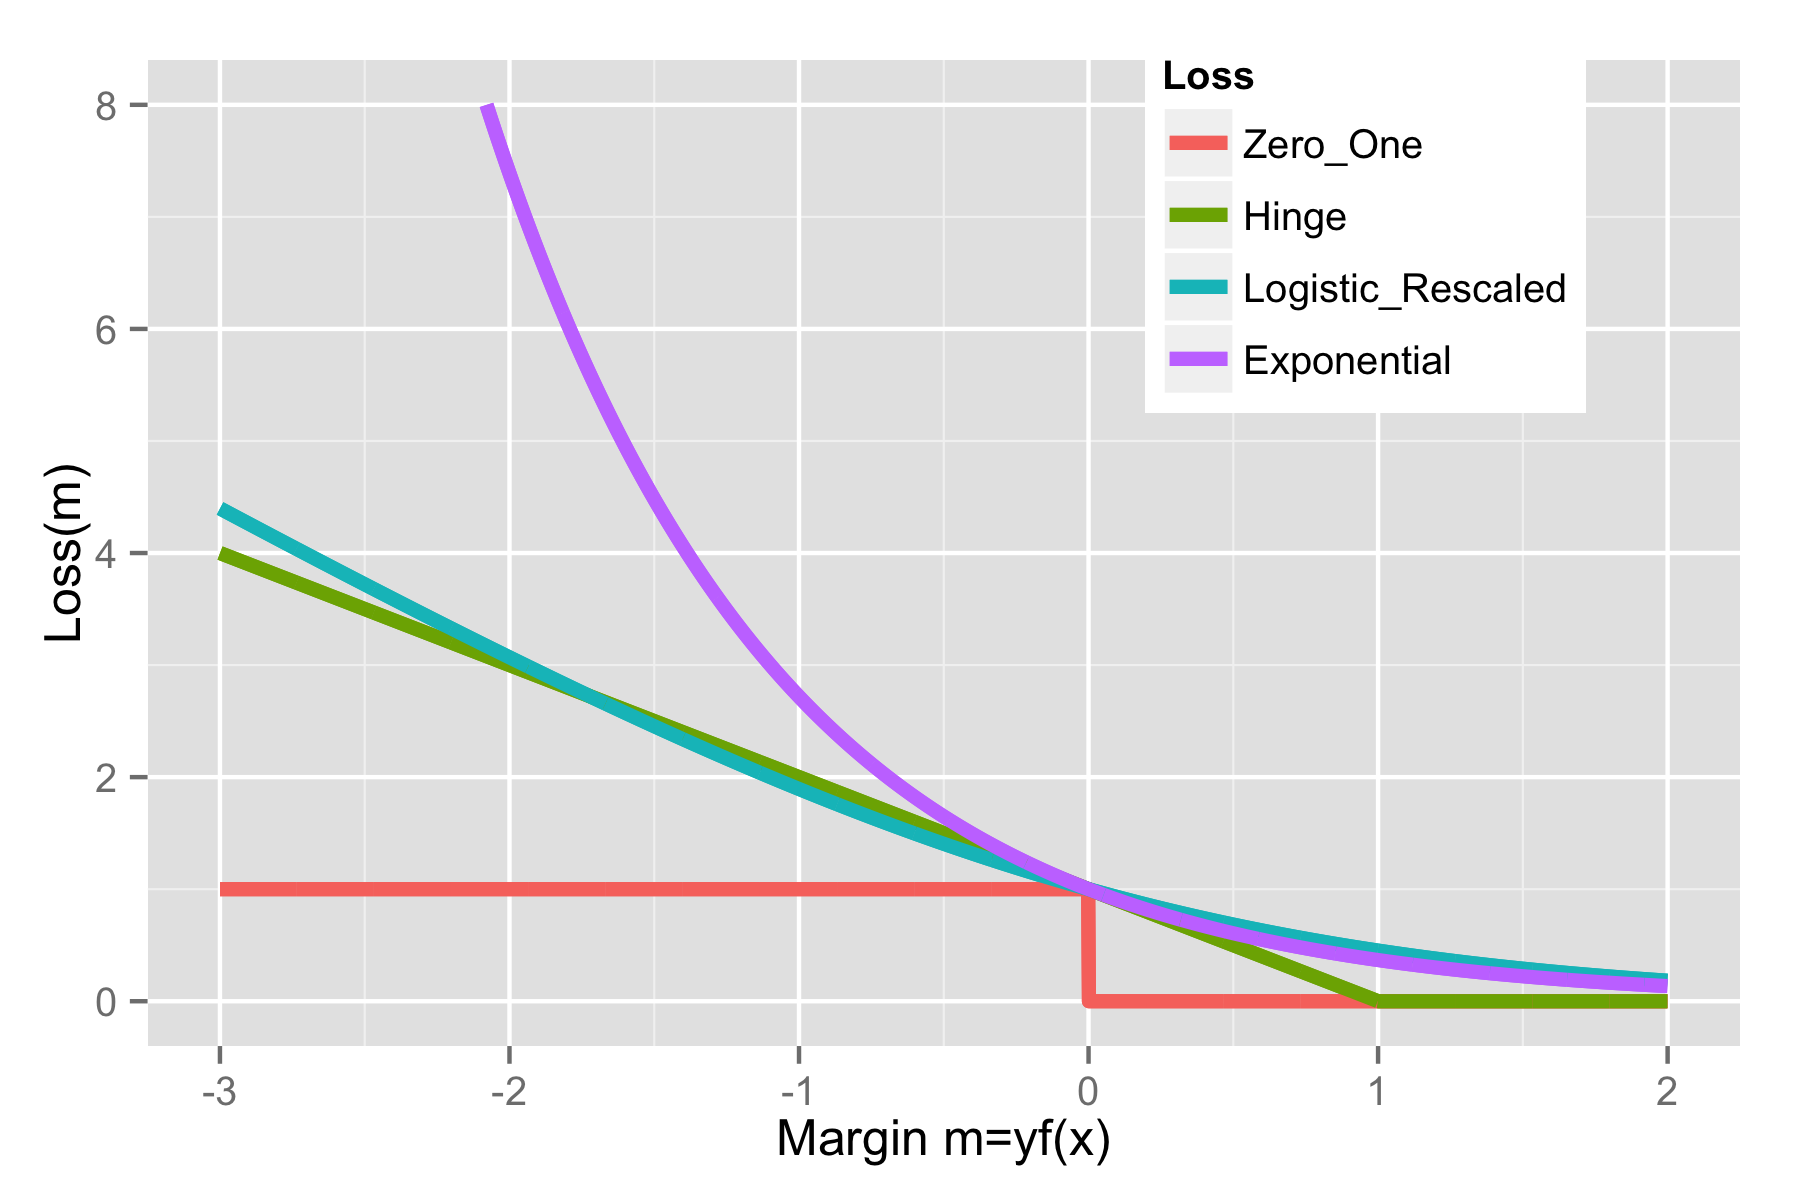
\includegraphics[height=0.45\textheight]{{figures/loss.Zero_One.Hinge.Logistic_Rescaled.Exponential}.png}
\end{center}
\end{itemize}
\note[item]{Adaboost was not initially designed to minimize exponential loss. It's only discovered 5 years after its invention. In the FSAM context, the main motivation for using exponential loss is computational: it leads to a simple optimization algorithm through example reweighting. But let's think about why this loss function makes sense from the statistical learning perspective.}
\note[item]{We can show that the optimal $f(x)$ is estimating one-half of the log odds. This justifies using the sign of it the make map the score to -1 and 1, \ie optimal under bayes decision rule.}
\note[item]{We have seen in logistic regression that its optimal estimate is also the log odds. So they will given the same model if there's infinite data. But in the finite-sample case, their behavior will be different.}
\note[item]{It puts more penalty on wrong predictions.}
\end{frame}
%
\begin{frame}{AdaBoost / Exponential Loss: Robustness Issues}
\begin{itemize}
\item Exponential loss puts a high penalty on misclassified examples.
\pause
\begin{itemize}
\item $\implies$ not robust to outliers / noise.
\end{itemize}
\item Empirically, AdaBoost has degraded performance in situations with 
\begin{itemize}
\item high Bayes error rate (intrinsic randomness in the label)
\end{itemize}
\pause
\item Logistic/Log loss performs better in settings with high Bayes error.
%\begin{itemize}
\item Exponential loss has some computational advantages over log loss though.
%\item FSAM + log loss $\implies$ LogitBoost
%\end{itemize}
\end{itemize}
\note[item]{Why is it bad? It means that the model will try very hard on a few misclassified examples.}
\end{frame}
%
\begin{frame}{Review}
We've seen
\begin{itemize}
\item Use basis function to obtain \emph{nonlinear} models: $f(x) = \sum_{i=1}^M v_m h_m(x)$ with known $h_m$'s.
\item \emph{Adaptive} basis function models: $f(x) = \sum_{i=1}^M v_m h_m(x)$ with unknown $h_m$'s.
\item Forward stagewise additive modeling: greedily fit $h_m$'s to minimize the average loss.
\end{itemize}
\pause
But,
\begin{itemize}
\item We only know how to do FSAM for certain loss functions.
\item Need to derive new algorithms for different loss functions.
\end{itemize}

Next, how to do FSAM in general.
\note[item]{Let's recap now. We started with the nonlinear regression problem. One way to obtain nonlinear classifier in the linear form is through basis functions, which compute a nonlinear transformation of $x$.}
\note[item]{If $h_m$ is known, that's easy---the problem is reduced to linear models. But what if we want to learn $h_m$'s?}
\note[item]{Last week we saw how to use the iterative Adaboost algorithm to find these base classifiers or basis functions. Today we saw that it's a special case of FSAM using exponential loss.}
\note[item]{In the FSAM framework, it is easy to plug in new loss functions.}
\end{frame}
%

\section{Gradient Boosting / ``Anyboost''}
\subsection{Motivating example: L2 Boosting}
\begin{frame}{FSAM with squared loss}
\begin{itemize}[<+->]
\item Objective function at $m$'th round:
\[
J(v,h)=\frac{1}{n}\sum_{i=1}^{n}\left(y_{i}-\left[f_{m-1}(x_{i})\underbrace{+v h(x_{i})}_{\text{new piece}}\right]\right)^{2}
\]

\item If $\ch$ is closed under rescaling (i.e. if $h\in\ch$, then $vh\in\ch$
for all $h\in\reals$), then don't need $v$.

\item Take $v=1$ and minimize
\[
J(h)=\frac{1}{n}\sum_{i=1}^{n}\left(\left[\underbrace{y_{i}-f_{m-1}(x_{i})}_{\onslide<+->{\text{residual}}}\right]-h(x_{i})\right)^{2}
\]

\item This is just fitting the residuals with least-squares regression!
\item<.-> Example base hypothesis space: regression stumps.
\end{itemize}
\note[item]{Let's consider FSAM with squared loss a s a motivating example.}
\note[item]{Remember that in each round of FSAM we minimize the empirical risk, which is the average loss on the training data. And we only fit one basis function without changing the previous ones.}
\note[item]{Now, we want to find $h$ in our base hypothesis space that minimizes $J$. First notice that if $\sH$ is closed under rescaling, meaning that if a function is in $\sH$ then its scaled version also belongs to $\sH$. Then we can consider $vh$ as another function $g$. Basically we can ignore $v$ if we assume...}
\note[item]{Now, let's re-arrange the terms. How do we interpret the first term?}
\note[item]{It's the residuals, so minimizing $J$ is equivalent to fit the residuals with squared loss.}
\end{frame}
%
%\begin{frame}{Regression Stumps}
%\begin{itemize}
%\item A \textbf{regression stump }is a regression tree with a single split.
%\item A\textbf{ regression stump }is a function of the form \textbf{$h(x)=a\ind{x_{i}\le c}+b\ind{x_{i}>c}$.}
%\end{itemize}
%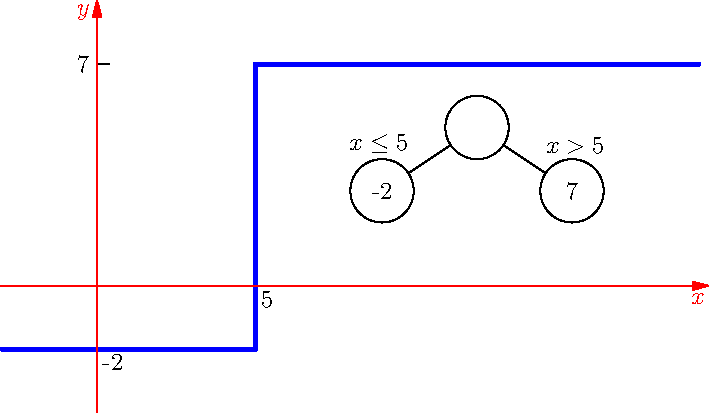
\includegraphics[clip,height=0.7\textheight]{figures/stump}
%\let\thefootnote\relax\footnotetext{\tiny{Plot courtesy of Brett Bernstein.}}
%\end{frame}
%%
\begin{frame}{$L^{2}$ Boosting with Decision Stumps: Demo}
\begin{itemize}
\item Consider FSAM with $L^{2}$ loss (i.e. $L^{2}$ Boosting)
\item For base hypothesis space of \textbf{regression stumps}
\end{itemize}

%\begin{itemize}
%\item Data we'll fit with \href{https://davidrosenberg.github.io/mlcourse/Labs/gbm.py}{code}:
%\end{itemize}
\begin{figure}
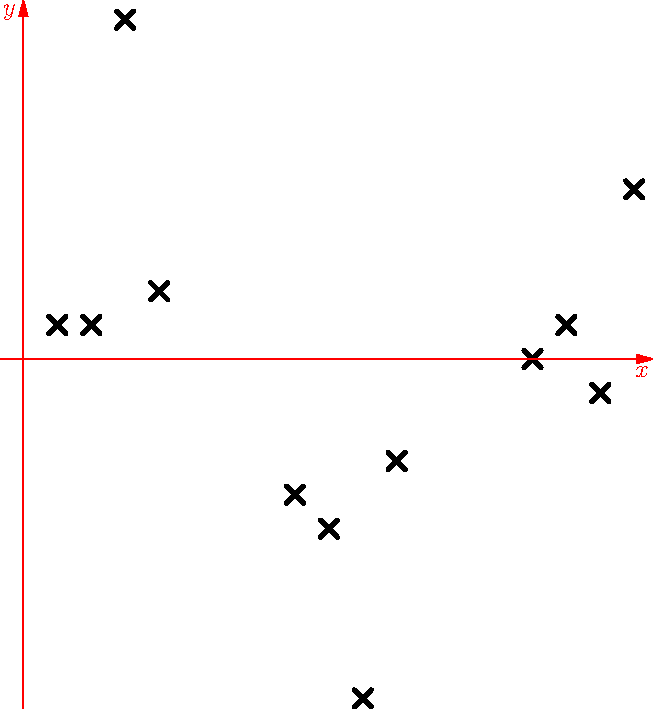
\includegraphics[clip,height=0.6\textheight]{figures/data}
\end{figure}

\let\thefootnote\relax\footnotetext{\tiny{Plot courtesy of Brett Bernstein.}}
\note[item]{Let's look at an example now to go over each round of FSAM with squared loss, which is also called L2 boosting. Our base hypothesis space is regression stumps, which is a regression tree with one split.}
\note[item]{Here's our data. Obviously it's non-linear.}
\end{frame}
%
\begin{frame}{$L^{2}$ Boosting with Decision Stumps: Results}
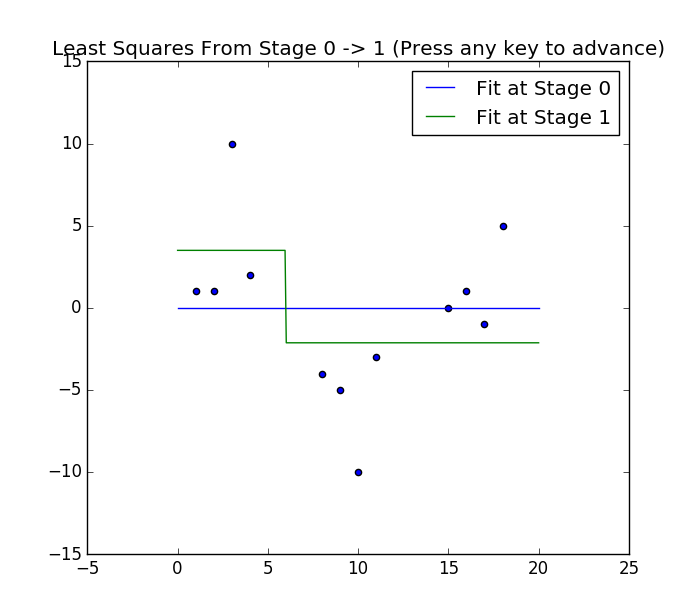
\includegraphics[height=0.8\textheight]{figures/l2boosting-stage1}%
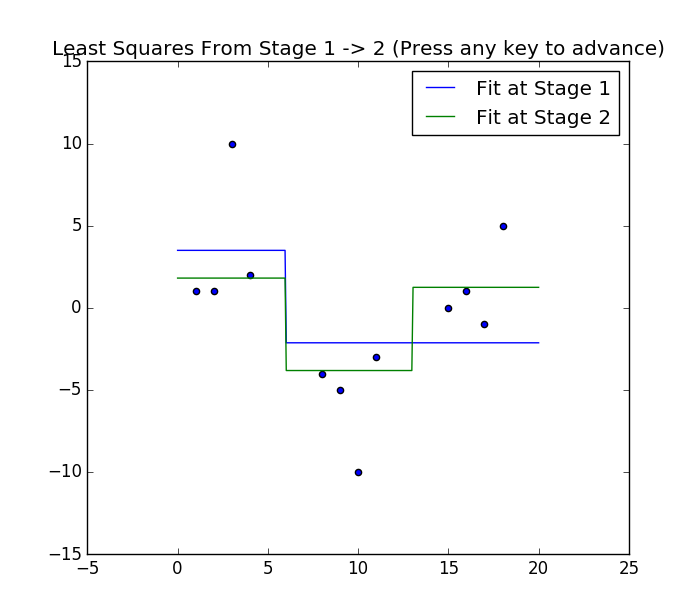
\includegraphics[height=0.8\textheight]{figures/l2boosting-stage2}
\let\thefootnote\relax\footnotetext{\tiny{Plots and code courtesy of Brett Bernstein.}}
\note[item]{Initially, our predictor is constant 0.}
\note[item]{Our first regression stump is the green line.}
\note[item]{In the next stage, we start with the sum of previous predictors, which is the blue line in the right figure.}
\note[item]{We add another decision stump which gives us the green line.}
\end{frame}
%
\begin{frame}{$L^{2}$ Boosting with Decision Stumps: Results}
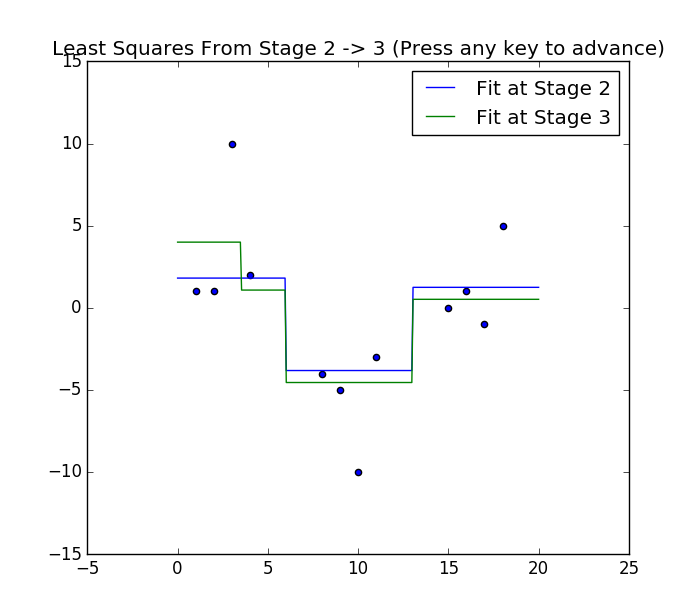
\includegraphics[height=0.8\textheight]{figures/l2boosting-stage3}%
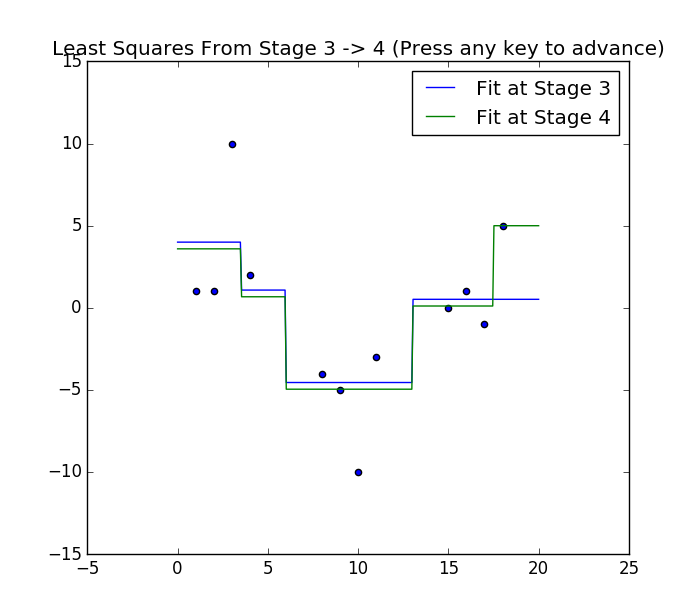
\includegraphics[height=0.8\textheight]{figures/l2boosting-stage4}
\let\thefootnote\relax\footnotetext{\tiny{Plots and code courtesy of Brett Bernstein.}}
\note[item]{So each time we add a new decision stump, so on and so forth.}
\end{frame}
%
\begin{frame}{$L^{2}$ Boosting with Decision Stumps: Results}

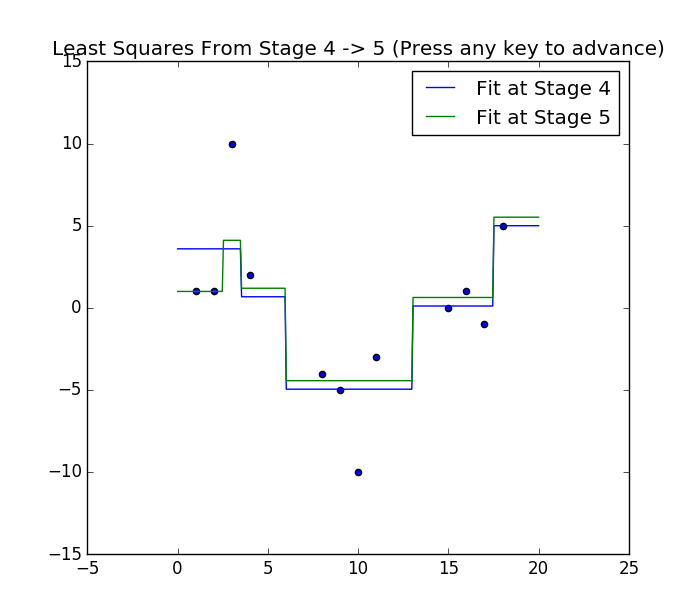
\includegraphics[height=0.8\textheight]{figures/l2boosting-stage5}%
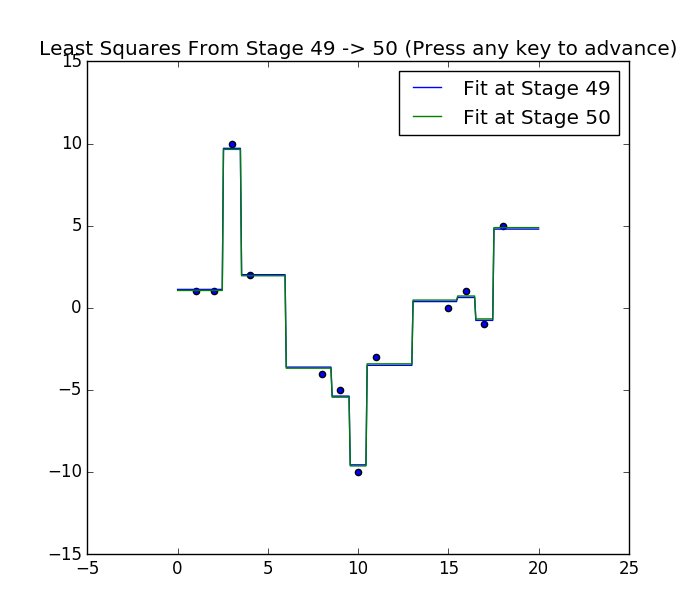
\includegraphics[height=0.8\textheight]{figures/l2boosting-stage50}
\let\thefootnote\relax\footnotetext{\tiny{Plots and code courtesy of Brett Bernstein.}}
\note[item]{After 50 stages, we can see that it overfitted. We will talk about how to prevent overfitting at the end.}
\note[item]{To summarize, in each round, we make a local improvement of our loss function. Specifically, here we move towards the target value incrementally. Now this process is actually quite similar to gradient descent, where we move along the direction that locally minimizes the objective. Next, let's consider its connection to gradient descent in a more formal way.}
\end{frame}

\begin{frame}
{Interpret the residual}
\begin{itemize}[<+->]
\item Objective: $J(f) = \frac{1}{n}\sum_{i=1}^n \p{y_i - f(x_i)}^2 $.
\item What is the residual at $x=x_i$?
\begin{align}
\frac{\partial}{\partial f(x_i)} J(f) = \onslide<+->{ -2 \p{y_i - f(x_i)} }
\end{align}
\begin{itemize}[<.->]
\item Gradient w.r.t. $f$: how should the output of $f$ change to minimize the squared loss.
\item \emph{Residual is the negative gradient} (differ by some constant).
\end{itemize}
\item At each boosting round, we learn a function $h\in\sH$ to fit the residual.
\begin{align}
f &\leftarrow f + {\color{red}v}{\color{Green}h} && \text{FSAM / boosting} \\
\onslide<+->{
f &\leftarrow f - {\color{red}\alpha}{\color{Green}\nabla_f J(f)} && \text{gradient descent}
}
\end{align}
\begin{itemize}[<.->]
\item $h$ approximates the gradient (step direction), $v$ is the step size.
\end{itemize}
\end{itemize}
\note[item]{So this is our loss function. Let's consider the value of $f$ at each training point $x_i$ as a variable that we can optimize.}
\note[item]{Then we can take gradient w.r.t. $f(x_i)$. That means how should we change the output at $x_i$ to minimize $J$.}
\note[item]{In FSAM, in each round we add a weighted basis function.}
\note[item]{Let's compare that with gradient descent. If we consider $f$ as a vector, then in each step, we move the vector along the negative gradient at the current value of $f$.}
\end{frame}

\subsection{Gradient Descent in the Function Space}

%\begin{frame}{FSAM Is Iterative Optimization}
%\begin{itemize}
%\item The FSAM step
%\[
%\left(v_{m},h_{m}\right)=\argmin_{v\in\reals,h\in\ch}\sum_{i=1}^{n}\ell\left(y_{i},f_{m-1}(x_{i})\underbrace{+v h(x_{i})}_{\text{new piece}}\right).
%\]
%
%
%\pause{}
%\item Hard part: finding the \textbf{best} \textbf{step direction} $h$.
%
%\pause{}
%\item What if we looked for the \textbf{locally best }step direction?
%\begin{itemize}
%\item like in gradient descent
%\end{itemize}
%\end{itemize}
%\end{frame}
%%
\begin{frame}{``Functional'' Gradient Descent }
\begin{itemize}
\item We want to minimize
\[
J(f)=\sum_{i=1}^{n}\ell\left(y_{i},f(x_{i})\right).
\]
\item In some sense, we want to take the gradient w.r.t. $f$.

\pause{}
\item $J(f)$ only depends on $f$ at the $n$ training points.

\pause{}
\item Define ``parameters''
\[
{\bf f}=\left(f(x_{1}),\ldots,f(x_{n})\right)^{T}
\]
and write the objective function as 
\[
J({\bf f})=\sum_{i=1}^{n}\ell\left(y_{i,}{\bf f}_{i}\right).
\]
\end{itemize}
\note[item]{We want to minimize $J$ w.r.t. the function $f$ by gradient descent, so the hard part is to compute the gradient, or the step direction.}
\note[item]{Notice that the objective only depends on the value of $f$ at $n$ points and doesn't really care about values elsewhere.}
\note[item]{So let's reformulate the problem by vectorizing $f$ into an $n$-dim vector. Now it becomes a familiar problem---we can easily take gradient w.r.t. this vector $f$.}
\end{frame}
%
\begin{frame}{Functional Gradient Descent: Unconstrained Step Direction}
\begin{itemize}[<+->]
\item Consider gradient descent on 
\[
J({\mathbf{f}})=\sum_{i=1}^{n}\ell\left(y_{i,}{\bf f}_{i}\right).
\]

\item The {negative gradient step direction} at ${\bf f}$ is
\begin{eqnarray*}
-{\bf g} & = & -\del_{\vf}J({\bf f})\\
 & = & -\left(\partial_{{\bf f}_{1}}\ell\left(y_{1},{\bf f}_{1}\right),\ldots,\partial_{{\bf f}_{n}}\ell\left(y_{n},{\bf f}_{n}\right)\right)
\end{eqnarray*}
which we can easily calculate.

\item<.-> $-{\bg}\in\reals^{n}$ is the direction we want to change each of
our $n$ predictions on training data.

\item With gradient descent, our final predictor will be an additive model: $f_0+\sum_{m=1}^M v_t (-\bg_t)$.
\end{itemize}

\note[item]{So what is our gradient now?}
\note[item]{The gradient is simply the vector of partial derivatives w.r.t. $f_i$'s. So now we have the direction towards which we can move our function $f$ at each training points.}
\note[item]{Starting with $f_0=0$, we will get an additive model with gradient descent.}
\end{frame}
%
\begin{frame}{Functional Gradient Descent: Projection Step}
\begin{itemize}[<+->]
\item Unconstrained step direction is
\[
-{\bg}=-\del_{\vf}J({\bf f})=-\left(\partial_{{\bf f}_{1}}\ell\left(y_{1},{\bf f}_{1}\right),\ldots,\partial_{{\bf f}_{n}}\ell\left(y_{n},{\bf f}_{n}\right)\right).
\]
\begin{itemize}[<.->]
\item Also called the ``\textbf{pseudo-residuals}''.
(For squared loss, they're exactly the residuals.)
\end{itemize}

\item 
\alarm{Problem}: only know how to update $\bf$ at $n$ points. How do we take a  gradient step in $\sH$?
\item \emph{Solution}: approximate by the closest base hypothesis $h\in\ch$ (in the $\ell^{2}$ sense):
\begin{align}
\min_{h\in\ch}\sum_{i=1}^{n}\left(-{\bf g}_{i}-h(x_{i})\right)^{2}.
&& \text{least square regression}
\end{align}

\item<.-> Take the $h\in\ch$ that best approximates $-{\bf g}$ as our step
direction.
\end{itemize}
\note[item]{However, our gradient is only defined on $n$ points. In other words, it is in $\reals^n$. But we want an update in the base hypothesis space. In other words, we want to project $g$ to $\sH$.}
\note[item]{So the problem now becomes finding a function in $\sH$ whose values at $x_i$'s are closest to the gradient vector, which is basically a regression problem.}
\end{frame}



\begin{frame}
{Recap}
\begin{itemize}[<+->]
\item Objective function: 
\begin{align}
J(f) = \sum_{i=1}^n \ell(y_i, f(x_i)) .
\end{align}
\item Unconstrained gradient $\bg \in \reals^n$ w.r.t. ${\vf}=(f(x_1), \ldots, f(x_n))^T$:
\begin{align}
{\bg}=\del_{\vf}J({\bf f})=\left(\partial_{{\bf f}_{1}}\ell\left(y_{1},{\bf f}_{1}\right),\ldots,\partial_{{\bf f}_{n}}\ell\left(y_{n},{\bf f}_{n}\right)\right).
\end{align}
\item Projected negative gradient $h \in \sH$:
\begin{align}
h = \argmin_{h\in\ch}\sum_{i=1}^{n}\left(-{\bf g}_{i}-h(x_{i})\right)^{2}.
\end{align}
\item Gradient descent:
\begin{align}
f \leftarrow f + {\color{red}v}h
\end{align}
\end{itemize}
\note[item]{But we still need to figure out the step size $v$.}
\end{frame}

\begin{frame}{Functional Gradient Descent: hyperparameters}
\begin{itemize}
\item Choose a step size by \textbf{line search}. 
\[
v_{m}=\argmin_{v}\sum_{i=1}^{n}\ell\left\{ y_{i},f_{m-1}(x_{i})+v h_{m}(x_{i})\right\} .
\]
\begin{itemize}
\item Not necessary. Can also choose a fixed hyperparameter $v$.
\end{itemize}
\item Regularization through \textbf{shrinkage}:
\begin{align}
f_m \leftarrow f_{m-1} + {\color{blue}\lambda} v_m h_m \quad \text{where}\; \lambda \in \pb{0,1} .
\end{align}
\begin{itemize}
\item Typically choose $\lambda = 0.1 $.
\end{itemize}

\item Choose $M$, \ie when to stop.
\begin{itemize}
\item Tune on validation set.
\end{itemize}
\end{itemize}
\note[item]{Now that we know $h_m$, we can solve another optimization problem to find the best $v_m$ that minimizes the objective.}
\note[item]{An alternative is to fix the step size, which can be tuned on the validation set.}
\end{frame}
%
\begin{frame}
{Gradient boosting algorithm}
\begin{enumerate}
\item Initialize $f$ to a constant: $f_0(x) = \argmin_\gamma \sum_{i=1}^n \ell(y_i, \gamma)$.
\item For $m$ from $1$ to $M$:
\begin{enumerate}
\item Compute the pseudo-residuals (negative gradient):
\begin{align}
r_{im} = -\pb{ \frac{\partial}{\partial f(x_i)} \ell(y_i, f(x_i) }_{f(x_i) = f_{m-1}(x_i)}
\end{align}
\item Fit a base learner $h_m$ with squared loss using the dataset $\pc{(x_i, r_{im})}_{i=1}^n$.
\item {[Optional]} Find the best step size $v_m = \argmin_v \sum_{i=1}^n \ell\p{yi, f_{m-1}(x_i) + vh_m(x_i)}.$
\item Update $f_m = f_{m-1} + \lambda v_mh_m$
\end{enumerate}
\item Return $f_M(x)$.
\end{enumerate}
\end{frame}

\begin{frame}{The Gradient Boosting Machine Ingredients (Recap)}
\begin{itemize}
\item Take any loss function {[}sub{]}differentiable w.r.t. the prediction $f(x_i)$
\item Choose a base hypothesis space for regression.
\item Choose number of steps (or a stopping criterion).
\item Choose step size methodology.
\item Then you're good to go!
\end{itemize}
\end{frame}
%

\subsection{Example: BinomialBoost}
\begin{frame}{BinomialBoost: Gradient Boosting with Logistic Loss}
\begin{itemize}
\item Recall the logistic loss for classification, with $\cy=\left\{ -1,1\right\} $:
\begin{eqnarray*}
\ell(y,f(x)) & = & \log\left(1+e^{-yf(x)}\right)
\end{eqnarray*}
\end{itemize}

\pause{}
\begin{itemize}
\item Pseudoresidual for $i$'th example is negative derivative of loss
w.r.t. prediction:
\begin{align}
r_{i} &= -\frac{\partial}{\partial f(x_i)} \ell(y_i, f(x_i)) \\ 
 &= -\frac{\partial}{\partial f(x_i)} \left[\log\left(1+e^{-y_{i}f(x_{i})}\right)\right]\\
 &= \frac{y_{i}e^{-y_{i}f(x_{i})}}{1+e^{-y_{i}f(x_{i})}}\\
 &= \frac{y_{i}}{1+e^{y_{i}f(x_{i})}}
\end{align}
\end{itemize}
\end{frame}
%
\begin{frame}{BinomialBoost: Gradient Boosting with Logistic Loss}
\begin{itemize}
\item Pseudoresidual for $i$th example:
\begin{eqnarray*}
r_{i} & = & -\frac{\partial}{\partial f(x_i)}\left[\log\left(1+e^{-y_{i}f(x_{i})}\right)\right]=\frac{y_{i}}{1+e^{y_{i}f(x_{i})}}
\end{eqnarray*}
\end{itemize}

\pause{}
\begin{itemize}
\item So if $f_{m-1}(x)$ is prediction after $m-1$ rounds, step direction
for $m$'th round is
\end{itemize}
\[
h_{m}=\argmin_{h\in\ch}\sum_{i=1}^{n}\left[\left(\frac{y_{i}}{1+e^{y_{i}f_{m-1}(x_{i})}}\right)-h(x_{i})\right]^{2}.
\]


\pause{}
\begin{itemize}
\item And $f_{m}(x)=f_{m-1}(x)+v h_{m}(x).$
\end{itemize}
\note[item]{This pseudo residuals are our targets of the function at $n$ points. So what's our regression problem?}
\end{frame}

\subsection{Gradient Tree Boosting}
\begin{frame}{Gradient Tree Boosting}
\begin{itemize}
\item One common form of gradient boosting machine takes
\[
\ch=\left\{ \mbox{regression trees of size \ensuremath{S}}\right\} ,
\]
where $S$ is the number of terminal nodes.

\item $S=2$ gives decision stumps

\item HTF recommends $4\le S\le8$ (but more recent results use much larger
trees)
\item Software packages:
\begin{itemize}
\item Gradient tree boosting is implemented by the {gbm package}
for R
\item as \texttt{\footnotesize{}GradientBoostingClassifier} and \texttt{\footnotesize{}GradientBoostingRegressor}
in {sklearn}
\item {xgboost} and {lightGBM} are state of the art for speed
and performance
\end{itemize}
\end{itemize}
\end{frame}

\begin{frame}{Sinc Function: Our Dataset}

\begin{figure}
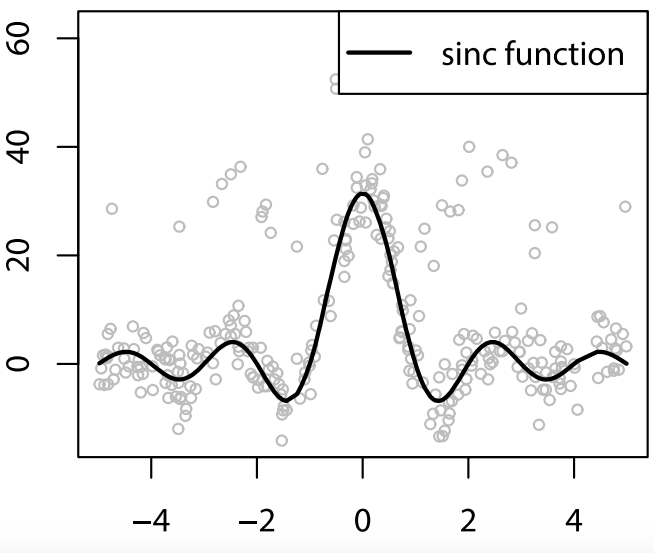
\includegraphics[height=0.6\textheight]{figures/sinc-fn-data}
\end{figure}

\let\thefootnote\relax\footnotetext{\tiny{From Natekin and Knoll's "Gradient boosting machines, a tutorial"}}
\end{frame}
%
\begin{frame}{Minimizing Square Loss with Ensemble of Decision Stumps}
\begin{center}
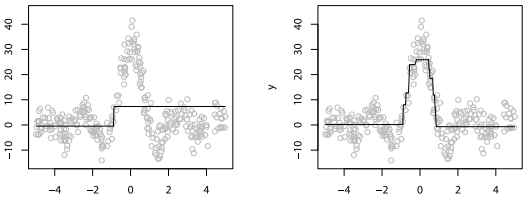
\includegraphics[height=0.3\textheight]{figures/sinc-fit-1step10steps}

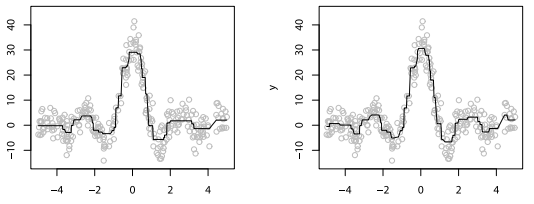
\includegraphics[height=0.3\textheight]{figures/sinc-fit-50steps100steps} 
\end{center}
Decision stumps with $1,10,50$, and $100$ steps, shrinkage $\lambda=1$.

\let\thefootnote\relax\footnotetext{\tiny{Figure 3 from Natekin and Knoll's "Gradient boosting machines, a tutorial"}}

\note[item]{A simple step function can be boosted to fit nonlinear data.}
\end{frame}
%

\section{Gradient Boosting in Practice}
\begin{frame}
{Prevent overfitting}
\begin{itemize}
\item Boosting is resistant to overfitting. Some explanations:
\begin{itemize}
\item Implicit feature selection: greedily selects the best feature (weak learner)
\item As training goes on, impact of change is localized.
\end{itemize}

\item But it can of course overfit. Common regularization methods:
\begin{itemize}
\item Shrinkage (small learning rate)
\item Stochastic gradient boosting (row subsampling)
\item Feature subsampling (column subsampling)
\end{itemize}
\end{itemize}
\end{frame}

\begin{frame}{Step Size as Regularization}

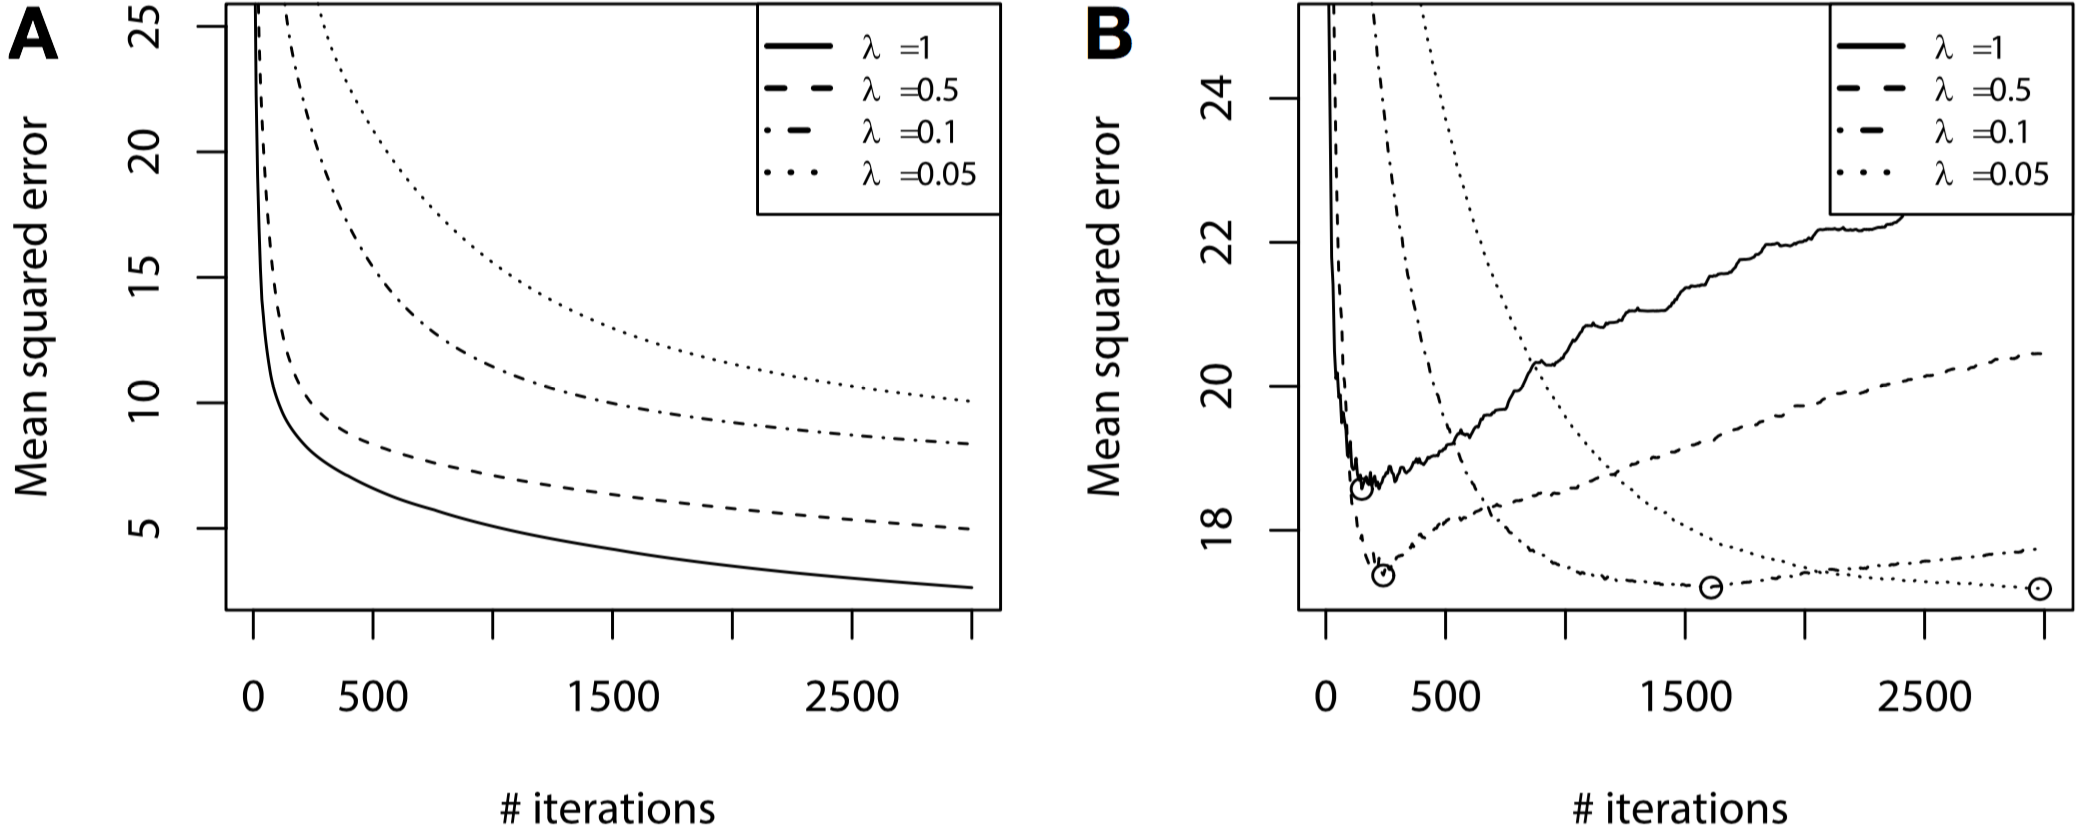
\includegraphics[width=0.8\textwidth]{figures/sinc-regression-train-validation} 

\begin{itemize}
\item (continued) sinc function regression
\item Performance vs rounds of boosting and shrinkage. (Left is training
set, right is validation set)
\end{itemize}

\let\thefootnote\relax\footnotetext{\tiny{Figure 5 from Natekin and Knoll's "Gradient boosting machines, a tutorial"}}
\note[item]{Left is training: larger step size leads to lower training loss as it updates more aggressively.}
\note[item]{Right is validation: larger step size converges faster but also converge to a worse solution.}
\end{frame}
%
\begin{frame}{Rule of Thumb}
\begin{itemize}
\item The smaller the step size, the more steps you'll need.
\item But never seems to make results worse, and often better.
\item So set your step size as small as you have patience for.
\end{itemize}
\note[item]{Next let's consider subsampling method.}
\end{frame}

\begin{frame}{Stochastic Gradient Boosting}
\begin{itemize}[<+->]
\item For each stage, 
\begin{itemize}[<.->]
\item choose random \emph{subset of data} for computing projected gradient step.
\end{itemize}
\item Why do this?
\begin{itemize}[<.->]
\item Introduce randomization thus may help overfitting.
\item Faster; often better than gradient descent given the same computation resource.
\end{itemize}
\item We can view this is a \textbf{minibatch method}. 
\begin{itemize}[<.->]
\item Estimate the ``true'' step direction
using a subset of data.
\end{itemize}
\let\thefootnote\relax\footnotetext{\tiny{Introduced by Friedman (1999) in \href{http://statweb.stanford.edu/~jhf/ftp/stobst.pdf}{Stochastic Gradient Boosting}. }}
\end{itemize}
\end{frame}
%
%\begin{frame}{Bag as Minibatch}
%\begin{itemize}
%\item Just as we argued for minibatch SGD, 
%\begin{itemize}
%\item sample size needed for a good estimate of step direction is independent
%of training set size
%\end{itemize}
%
%\pause{}
%\item Minibatch size should depend on 
%\begin{itemize}
%\item the complexity of base hypothesis space
%\item the complexity of the target function (Bayes decision function)
%\end{itemize}
%
%\pause{}
%\item Seems like an interesting area for both practical and theoretical
%pursuit.
%\end{itemize}
%\end{frame}
%

\begin{frame}{Column / Feature Subsampling}
\begin{itemize}
\item Similar to random forest, randomly choose \emph{a subset of features} for
each round.

\item XGBoost paper says: ``According to user feedback, using column sub-sampling
prevents overfitting even more so than the traditional row sub-sampling.''

\item Speeds up computation.
\end{itemize}
\end{frame}

%\begin{frame}{Newton Step Direction}
%\begin{itemize}
%\item For GBM, we find the closest $h\in\cf$ to the negative gradient
%\[
%-{\bf g}=-\del_{\vf}J({\bf f}).
%\]
%\item This is a ``first order'' method. 
%\end{itemize}
%
%\pause{}
%\begin{itemize}
%\item Newton's method is a ``second order method'':
%\begin{itemize}
%\item Find 2nd order (quadratic) approximation to $J$ at $\vf$.
%\begin{itemize}
%\item Requires computing gradient and Hessian of $J$.
%\end{itemize}
%\item Newton step direction points towards minimizer of the quadratic.
%\item Minimizer of quadratic is easy to find in closed form
%\end{itemize}
%
%\pause{}
%\item Boosting methods with projected Newton step direction:
%\begin{itemize}
%\item LogitBoost (logistic loss function)
%\item XGBoost (any loss \textendash{} uses regression trees for base classifier)
%\end{itemize}
%\end{itemize}
%\end{frame}
%%
%\begin{frame}{Newton Step Direction for GBM}
%\begin{itemize}
%\item Generically, second order Taylor expansion of $J$ at ${\bf f}$ in
%direction ${\bf r}$
%\[
%J({\bf f}+{\bf r})=J({\bf f})+\left[\del_{{\bf f}}J({\bf f})\right]^{T}{\bf r}+\frac{1}{2}{\bf r}^{T}\left[\del_{{\bf f}}^{2}J({\bf f})\right]{\bf r}
%\]
%
%
%\pause{}
%\item For $J({\bf f})=\sum_{i=1}^{n}\ell\left(y_{i},{\bf f}_{i}\right)$,
%\[
%J({\bf f}+{\bf r})=\sum_{i=1}^{n}\left[\ell\left(y_{i},{\bf f}_{i}\right)+g_{i}{\bf r}_{i}+\frac{1}{2}h_{i}{\bf r}_{i}^{2}\right],
%\]
%where $g_{i}=\partial_{{\bf f}_{i}}\ell\left(y_{i},{\bf f}_{i}\right)$
%and $h_{i}=\partial_{{\bf f}_{i}}^{2}\ell\left(y_{i},{\bf f}_{i}\right)$. 
%
%\pause{}
%\item Can find ${\bf r}$ that minimizes $J({\bf f}+{\bf r})$ in closed
%form. 
%
%\pause{}
%\item Can take step direction to be ``projection'' of ${\bf r}$ into
%base hypothesis space $\ch$.
%\end{itemize}
%\end{frame}

\begin{frame}
{Summary}
\begin{itemize}
\item Motivating idea of boosting: combine weak learners to produce a strong learner.
\item The statistical view: boosting is fitting an additive model (greedily).
\item The numerical optimization view: boosting makes local improvement iteratively---gradient descent in the function space.
\item Gradient boosting is a generic framework
\begin{itemize}
\item Any differentiable loss function
\item Classification, regression, ranking, multiclass etc.
\item Scalable, \eg XGBoost
\end{itemize}
\end{itemize}
\note[item]{We introduced boosting and Adaboost as an ensemble method in addition to bagging.}
\note[item]{But now we know that they are fundamentally very different ideas. The ensemble form of the final predictor is only a superficial connection.}
\note[item]{Boosting is fitting an additive model which aims to reduce bias, whereas often ensemble is meant to reduce variance.}
\note[item]{We can further generalize that to any loss function by functional gradient descent, or gradient boosting.}
\note[item]{In this lecture, we have seen how boosting started with a theoretical question and now produces large-scale system such as XGBoost used widely in practice. This is actually quite amazing.}
\end{frame}


\end{document}
